\clearpage

\section{SYSTEM ANALYSIS}

System analysis establishes the functional requirements, dataset architecture, preprocessing steps, exploratory data analysis, and algorithmic framework for the medical specialty classification system.

The Kaggle Medical Transcriptions (MTSamples) dataset, sourced from Kaggle \cite{mtsamples_dataset}, provides clinical narrative dictations across multiple healthcare sub-disciplines, enabling comprehensive evaluation of natural language processing and machine learning models for medical document categorization.

\textbf{Dataset Link}: \url{https://www.kaggle.com/datasets/tboyle10/medicaltranscriptions}

\textbf{Size}: The dataset comprises 4,999 clinical records spanning 40 distinct medical specialties.

\textbf{Data Structure}: It contains six attributes including row index (\texttt{Unnamed: 0}), short report abstract (\texttt{description}), target medical department (\texttt{medical\_specialty}), sample dictation title (\texttt{sample\_name}), main clinical narrative (\texttt{transcription}), and extracted key terms (\texttt{keywords}).

\textbf{Sparsity}: The primary text column (\texttt{transcription}) is highly complete, containing 33 missing records (0.66\%), which are dropped during preprocessing. The target label (\texttt{medical\_specialty}) contains zero missing values.

\subsection{EXPLORATORY DATA ANALYSIS}

\subsubsection{ABOUT THE DATASET}

\paragraph{Dataset Overview}
The Kaggle Medical Transcriptions dataset provides authentic clinical narratives dictating patient histories, diagnostic evaluations, physical examinations, and surgical procedures:
\begin{itemize}
    \item Total Records: 4,999 clinical reports.
    \item Total Features: 5 independent variables + 1 target variable (\texttt{medical\_specialty}).
    \item Data Types: Textual narratives (\texttt{transcription}, \texttt{description}, \texttt{keywords}), categorical labels (\texttt{medical\_specialty}), and integer index.
    \item Missing Values: Present in \texttt{description} (6 records), \texttt{transcription} (33 records), and \texttt{keywords} (1,068 records).
\end{itemize}

Table \ref{tab:dataset_summary_card} summarizes the core dataset attributes.

\begin{table}[H]
\centering
\small
\setlength{\tabcolsep}{5pt}
\begin{tabularx}{\linewidth}{|>{\raggedright\arraybackslash}p{3.8cm}|>{\raggedright\arraybackslash}X|}
\hline
\textbf{Property} & \textbf{Description} \\
\hline
\textbf{Dataset Name} & Kaggle Medical Transcriptions (MTSamples) Dataset \\
\hline
\textbf{Source} & Kaggle (\url{https://www.kaggle.com/datasets/tboyle10/medicaltranscriptions}) \\
\hline
\textbf{Total Records} & 4,999 clinical reports \\
\hline
\textbf{Number of Columns} & 6 fields (\texttt{Unnamed: 0}, \texttt{description}, \texttt{medical\_specialty}, \texttt{sample\_name}, \texttt{transcription}, \texttt{keywords}) \\
\hline
\textbf{Input Variable} & \texttt{transcription} (Primary clinical narrative text) \\
\hline
\textbf{Target Variable} & \texttt{medical\_specialty} (40 unique clinical specialties) \\
\hline
\textbf{Advantages} & Authentic clinical dictations; complete target label annotations (0 missing labels); broad multi-class domain coverage \\
\hline
\textbf{Limitations} & Severe class imbalance across categories; 33 missing transcriptions; 1,068 missing keyword entries; variable text length \\
\hline
\end{tabularx}
\caption{Characteristics of the Kaggle Medical Transcriptions Dataset}
\label{tab:dataset_summary_card}
\end{table}

The dataset attributes are categorized as follows:
\begin{enumerate}
    \item \textbf{Primary Clinical Narrative (\texttt{transcription})}: The central predictor attribute containing unstructured, dictation-style medical reports that detail symptoms, findings, diagnoses, and treatments.
    \item \textbf{Clinical Abstract (\texttt{description})}: Short one-to-two sentence summary of the clinical consultation or procedure.
    \item \textbf{Extracted Keywords (\texttt{keywords})}: Comma-delimited clinical terms and anatomical references extracted from the narrative.
    \item \textbf{Sample Identification (\texttt{sample\_name})}: Dictation title indicating the type of procedure or medical note.
    \item \textbf{Target Variable (\texttt{medical\_specialty})}: The multi-class categorical label representing the specialized department (40 clinical specialties).
\end{enumerate}

\subsubsection{STATISTICAL ANALYSIS}
Data exploration was conducted using Python data analysis tools (\texttt{pandas}, \texttt{numpy}). Inspection via \texttt{shape}, \texttt{info()}, \texttt{dtypes}, and \texttt{describe()} confirmed that the dataset contains 4,999 records and 6 columns without structural corruption. Table \ref{tab:column_description} describes each column, its data type, and missing value counts.

\begin{table}[H]
\centering
\small
\setlength{\tabcolsep}{5pt}
\begin{tabularx}{\linewidth}{|>{\raggedright\arraybackslash}p{3.0cm}|>{\raggedright\arraybackslash}p{2.0cm}|>{\raggedright\arraybackslash}X|r|}
\hline
\textbf{Column Name} & \textbf{Data Type} & \textbf{Description} & \textbf{Missing Count} \\
\hline
\texttt{Unnamed: 0} & Integer & Record Identifier / Row Index & 0 \\
\hline
\texttt{description} & Text & Short summary of clinical report & 6 \\
\hline
\texttt{medical\_specialty} & Categorical & Target specialty label (40 classes) & 0 \\
\hline
\texttt{sample\_name} & Text & Report title / dictation sample title & 0 \\
\hline
\texttt{transcription} & Text & Primary clinical narrative (Input) & 33 \\
\hline
\texttt{keywords} & Text & Extracted key terms & 1,068 \\
\hline
\end{tabularx}
\caption{Dataset Column Descriptions and Missing Value Audit}
\label{tab:column_description}
\end{table}

Descriptive statistical analysis revealed significant variation in class distribution across the 40 medical specialties. Table \ref{tab:top_bottom_specialties} lists the record counts for the top 10 majority specialties alongside the 10 rarest minority specialties.

\begin{table}[H]
\centering
\small
\setlength{\tabcolsep}{5pt}
\begin{tabularx}{\linewidth}{|>{\raggedright\arraybackslash}X|r|>{\raggedright\arraybackslash}X|r|}
\hline
\textbf{Top 10 Specialties} & \textbf{Count} & \textbf{Bottom 10 Specialties} & \textbf{Count} \\
\hline
Surgery & 1,103 & Cosmetic / Plastic Surgery & 27 \\
\hline
Consult - History and Phy. & 516 & Pediatric / Neonatal & 22 \\
\hline
Cardiovascular / Pulmonary & 372 & Sleep Medicine & 20 \\
\hline
Orthopedic & 355 & Bariatrics & 18 \\
\hline
Radiology & 273 & Speech - Language & 9 \\
\hline
General Medicine & 259 & Lab Medicine - Pathology & 8 \\
\hline
Gastroenterology & 230 & Allergy / Immunology & 7 \\
\hline
Neurology & 223 & Hospice - Palliative Care & 6 \\
\hline
SOAP / Chart / Progress Notes & 166 & Executive Evaluation & 2 \\
\hline
Obstetrics / Gynecology & 160 & Autopsy & 2 \\
\hline
\end{tabularx}
\caption{Distribution of Top 10 Majority and Bottom 10 Minority Medical Specialties}
\label{tab:top_bottom_specialties}
\end{table}

Statistical analysis of narrative text lengths indicated a positively skewed distribution. While the median document length is approximately 350 to 500 words, certain comprehensive operative notes and consultative evaluations extend beyond 2,000 words, necessitating length-normalization via TF-IDF vectorization.

\clearpage

\subsection{DATA VISUALIZATION}

Data visualization is an important stage of Exploratory Data Analysis (EDA) that helps in understanding the characteristics, distributions, and relationships among clinical narratives and medical specialties. Visual representations provide valuable insights into the dataset, reveal hidden patterns, and assist in verifying the suitability of the text data for machine learning classification.

\paragraph{Missing Value Analysis}
Figure \ref{fig:eda_missing} illustrates the distribution of missing values across dataset attributes. As shown, the primary target attribute (\texttt{medical\_specialty}) contains zero missing values. The primary input text narrative (\texttt{transcription}) contains 33 missing records, while the auxiliary \texttt{keywords} attribute exhibits 1,068 missing records.

\begin{figure}[H]
\centering
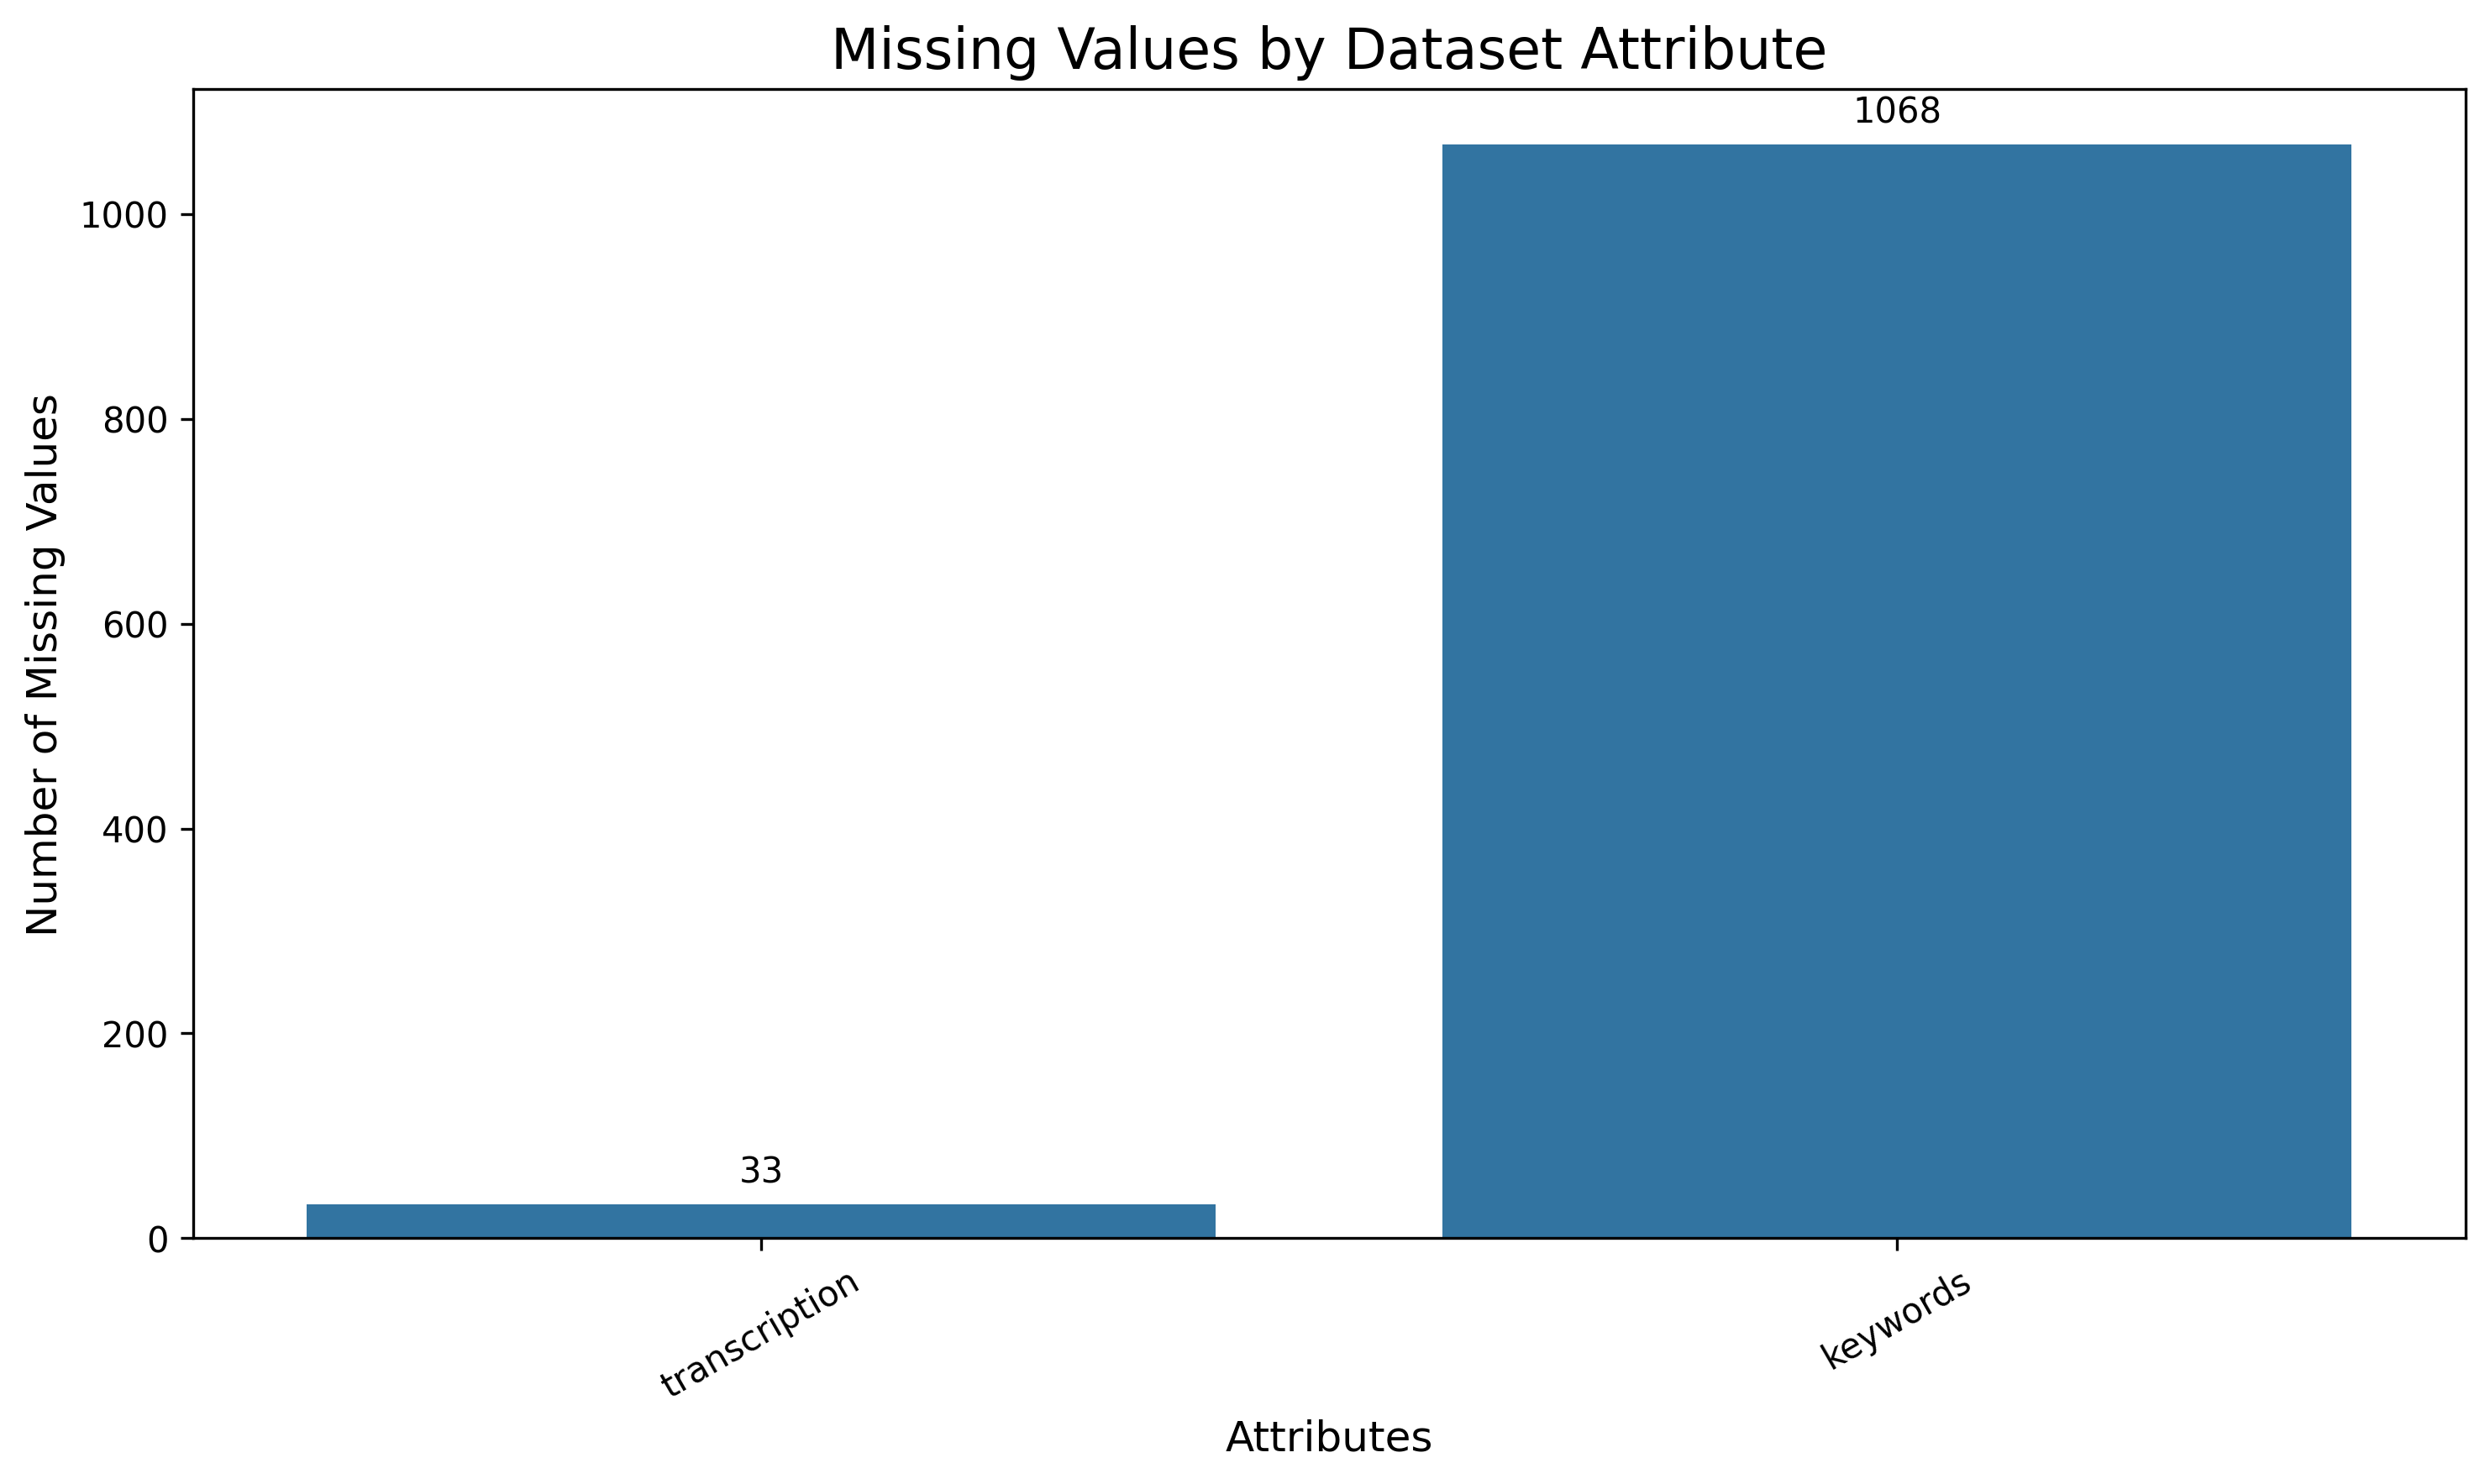
\includegraphics[width=0.82\textwidth,height=6.0cm,keepaspectratio]{EDA_Diagrams/01_missing_values.png}
\caption{Missing Values by Dataset Attribute}
\label{fig:eda_missing}
\end{figure}

\paragraph{Top 10 Medical Specialties}
Figure \ref{fig:eda_top10} displays the record counts for the top 10 medical specialties in the dataset. Surgery represents the single largest category with 1,103 clinical reports, followed by Consult - History and Phy. (516 reports), Cardiovascular / Pulmonary (372 reports), and Orthopedic (355 reports).

\begin{figure}[H]
\centering
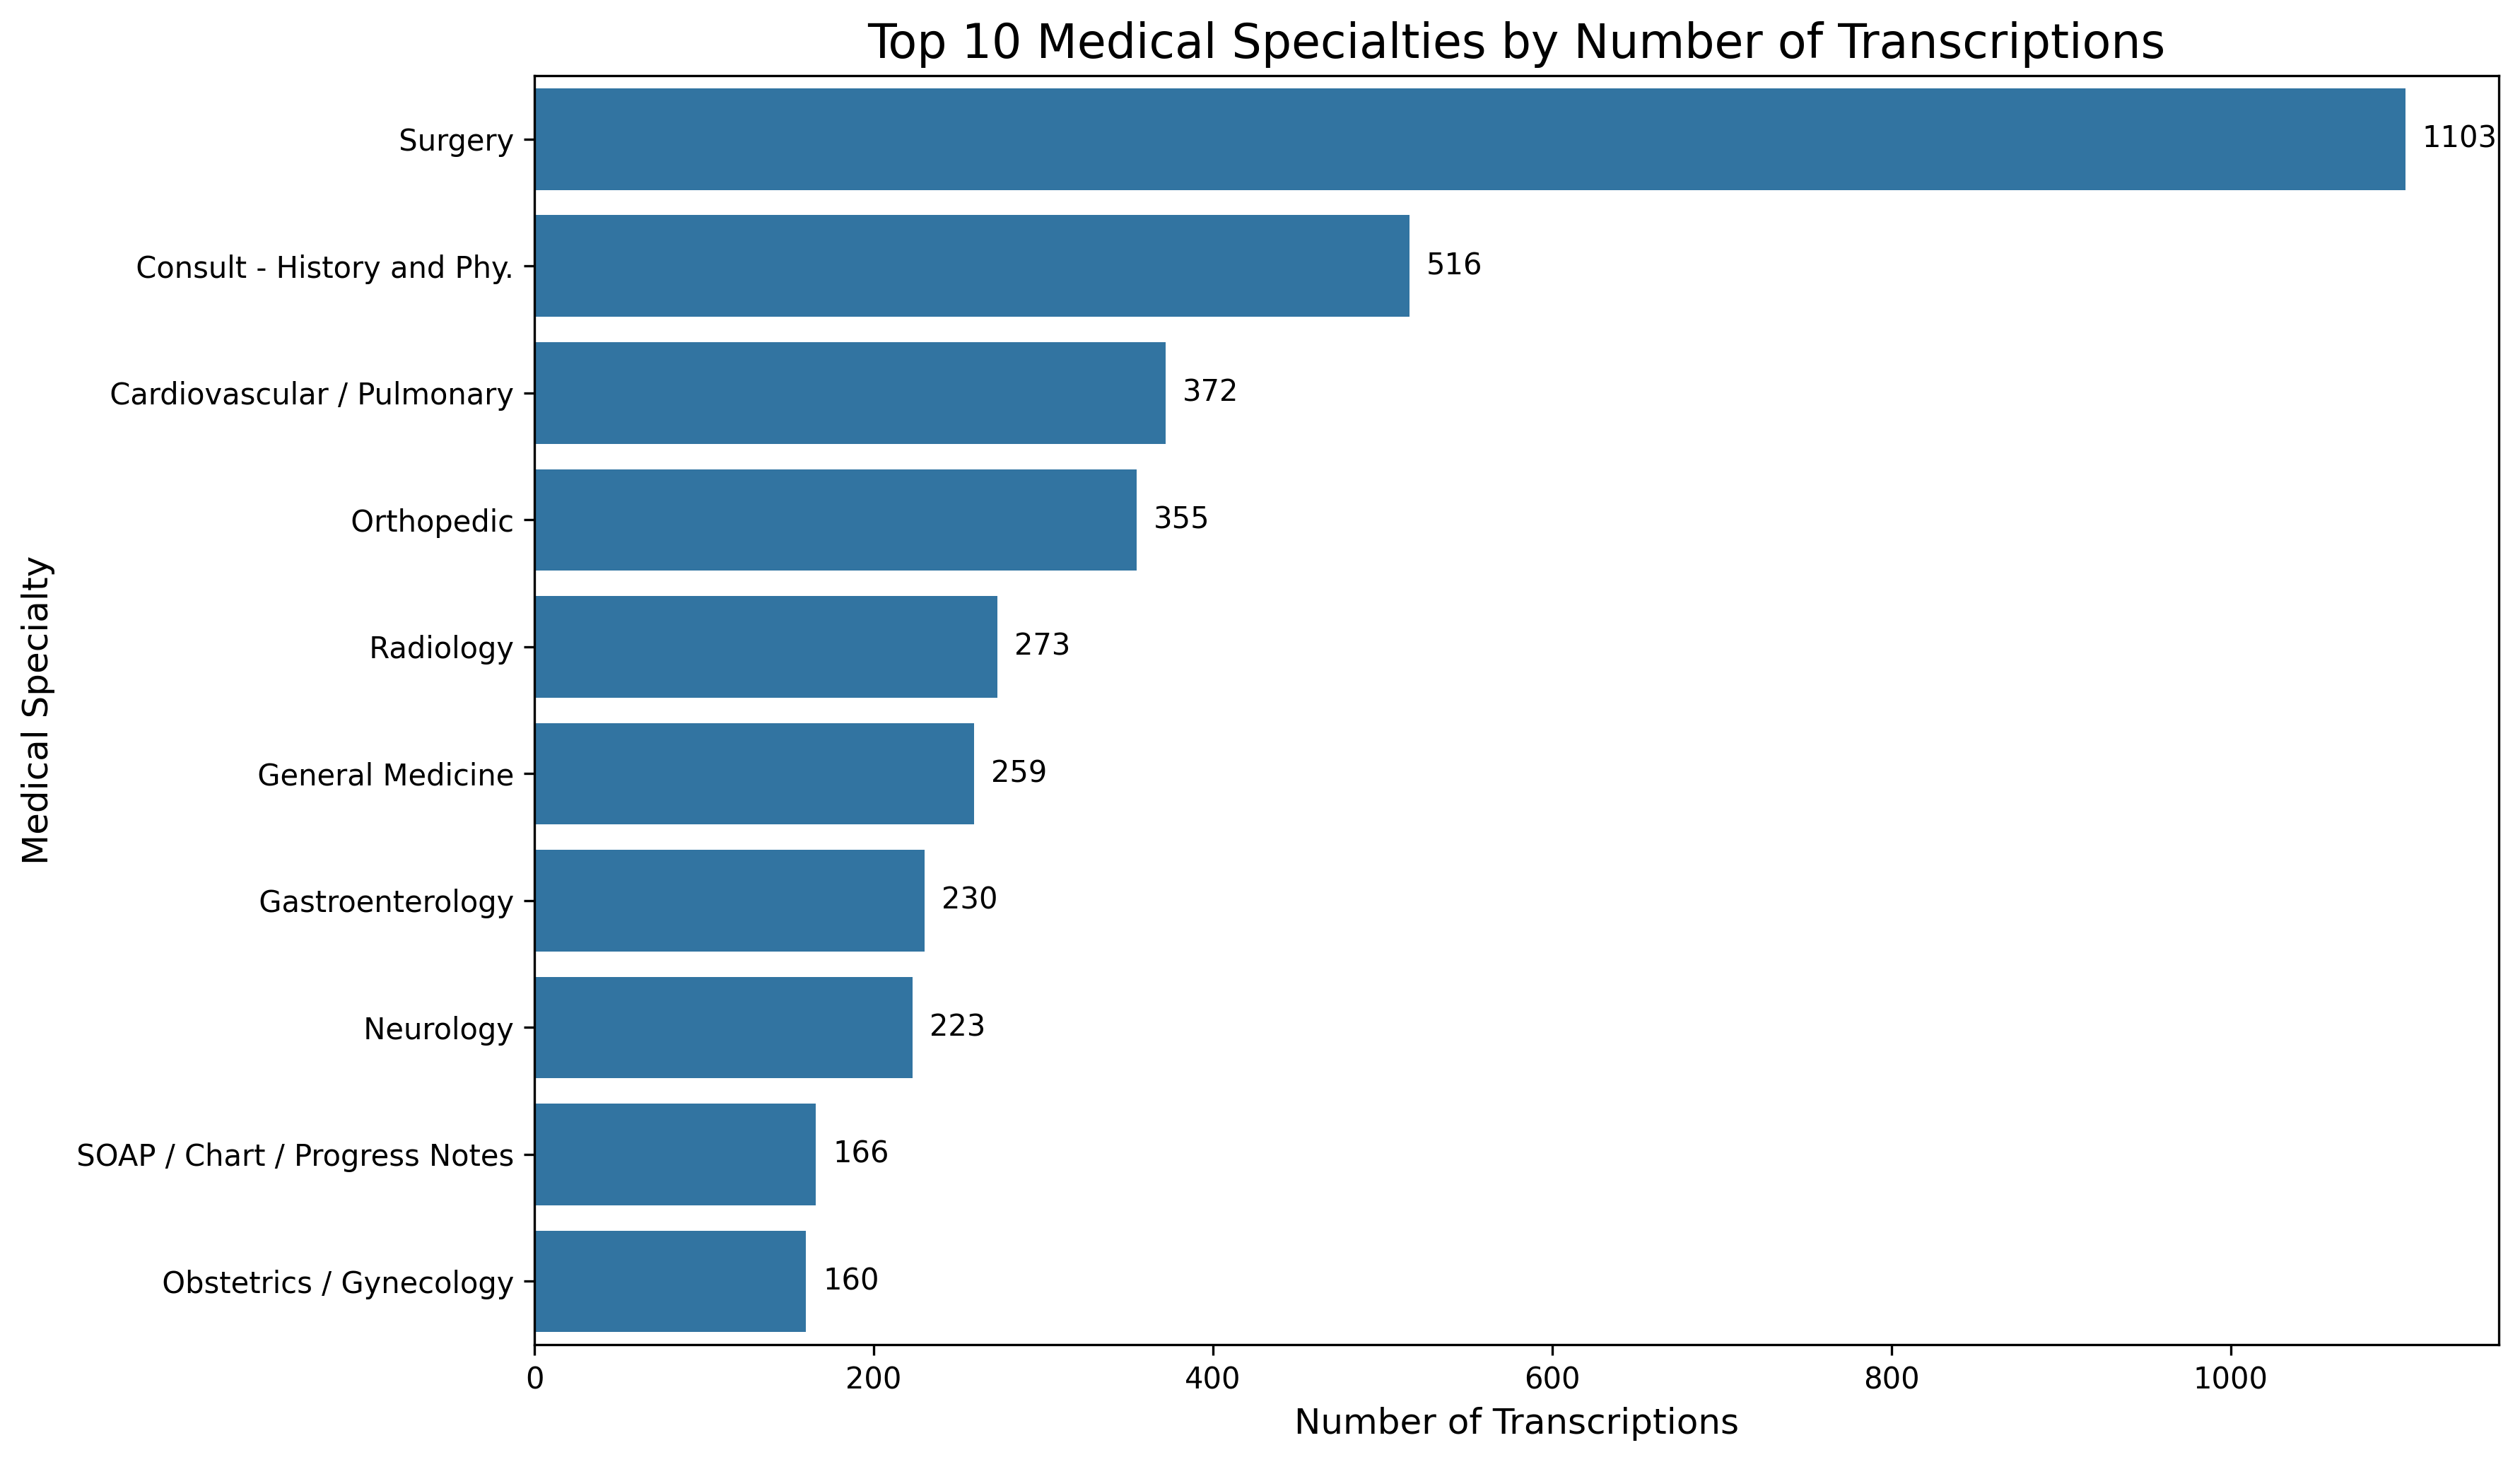
\includegraphics[width=0.82\textwidth,height=6.5cm,keepaspectratio]{EDA_Diagrams/02_top10_medical_specialties.png}
\caption{Top 10 Medical Specialties by Number of Transcriptions}
\label{fig:eda_top10}
\end{figure}

\paragraph{Complete Specialty Distribution}
Figure \ref{fig:eda_complete_specialty} illustrates the full class distribution across all 40 medical specialties in the MTSamples corpus. The chart demonstrates severe class imbalance, ranging from majority classes such as Surgery (1,103 records) down to highly specialized minority classes such as Hospice - Palliative Care, Allergy / Immunology, Lab Medicine - Pathology, and Autopsy with under 10 records each.

\begin{figure}[H]
\centering
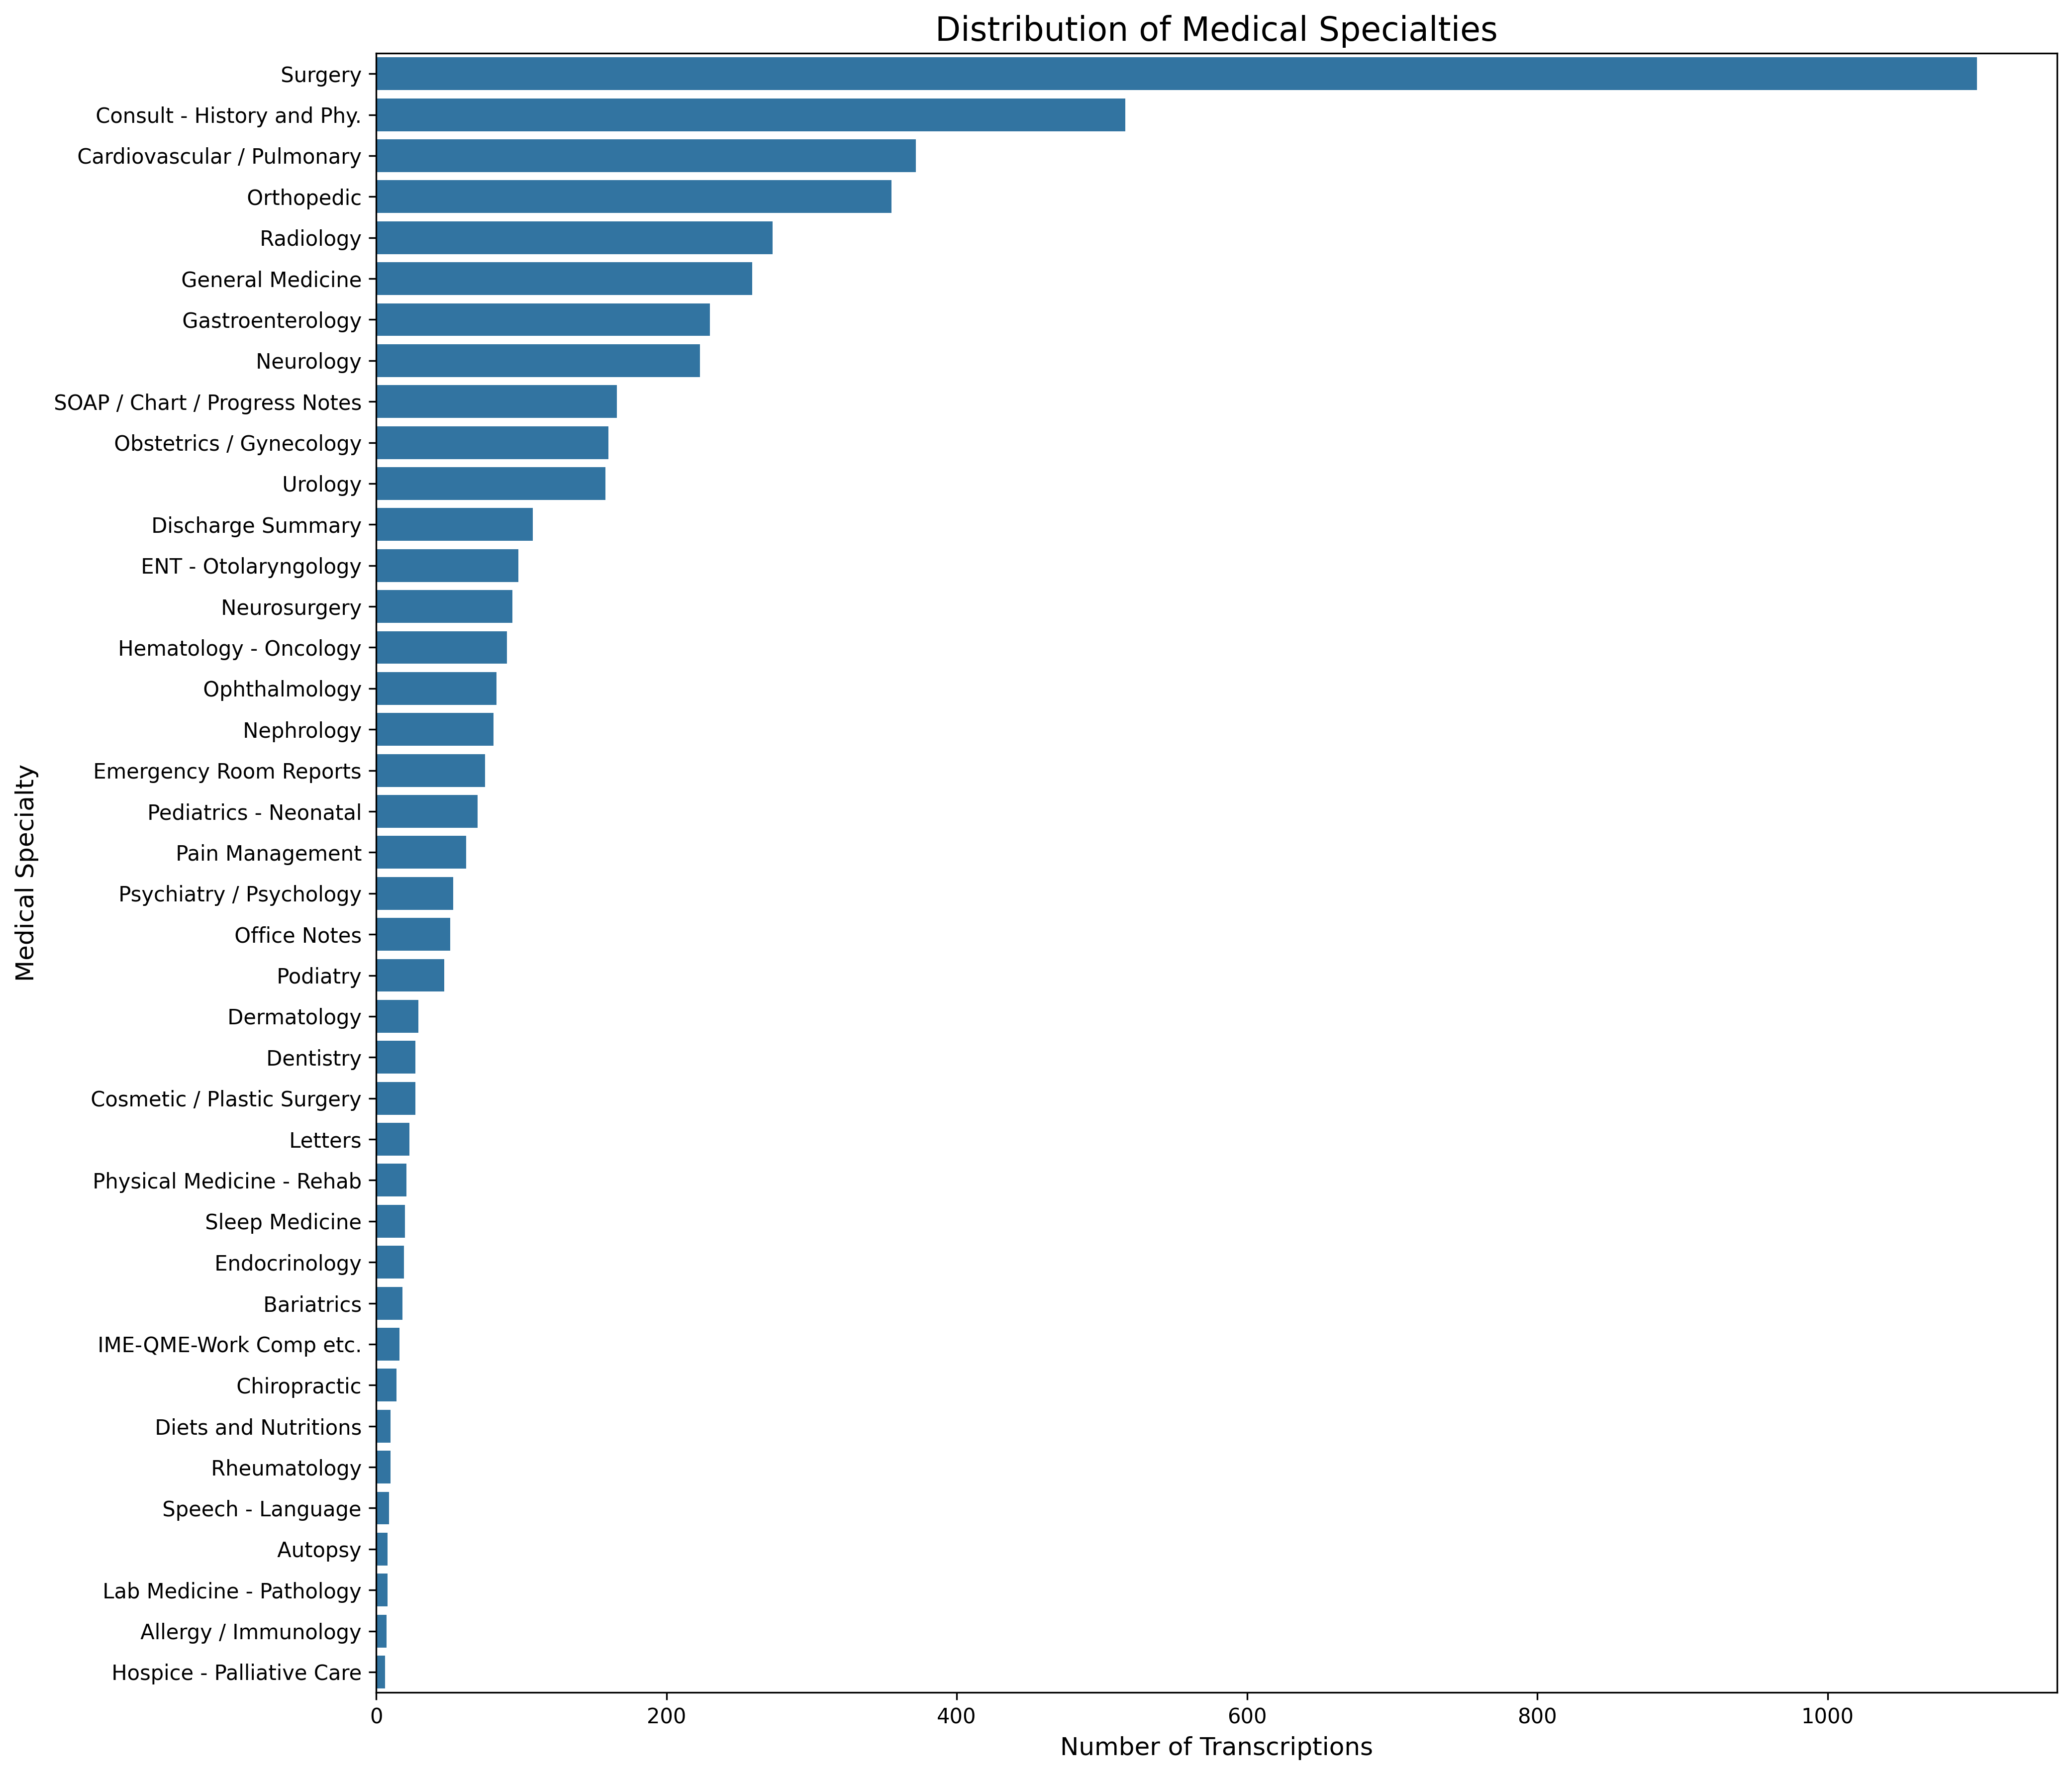
\includegraphics[width=0.82\textwidth,height=7.0cm,keepaspectratio]{EDA_Diagrams/03_complete_specialty_distribution.png}
\caption{Distribution of Medical Specialties}
\label{fig:eda_complete_specialty}
\end{figure}

\paragraph{Transcription Length Distribution}
Figure \ref{fig:eda_length_dist} displays the word count distribution for clinical narratives, fitted with a Kernel Density Estimate (KDE) curve. The majority of medical transcriptions range between 200 and 600 words, exhibiting a right-skewed distribution with extended narratives reaching up to 3,000 words.

\begin{figure}[H]
\centering
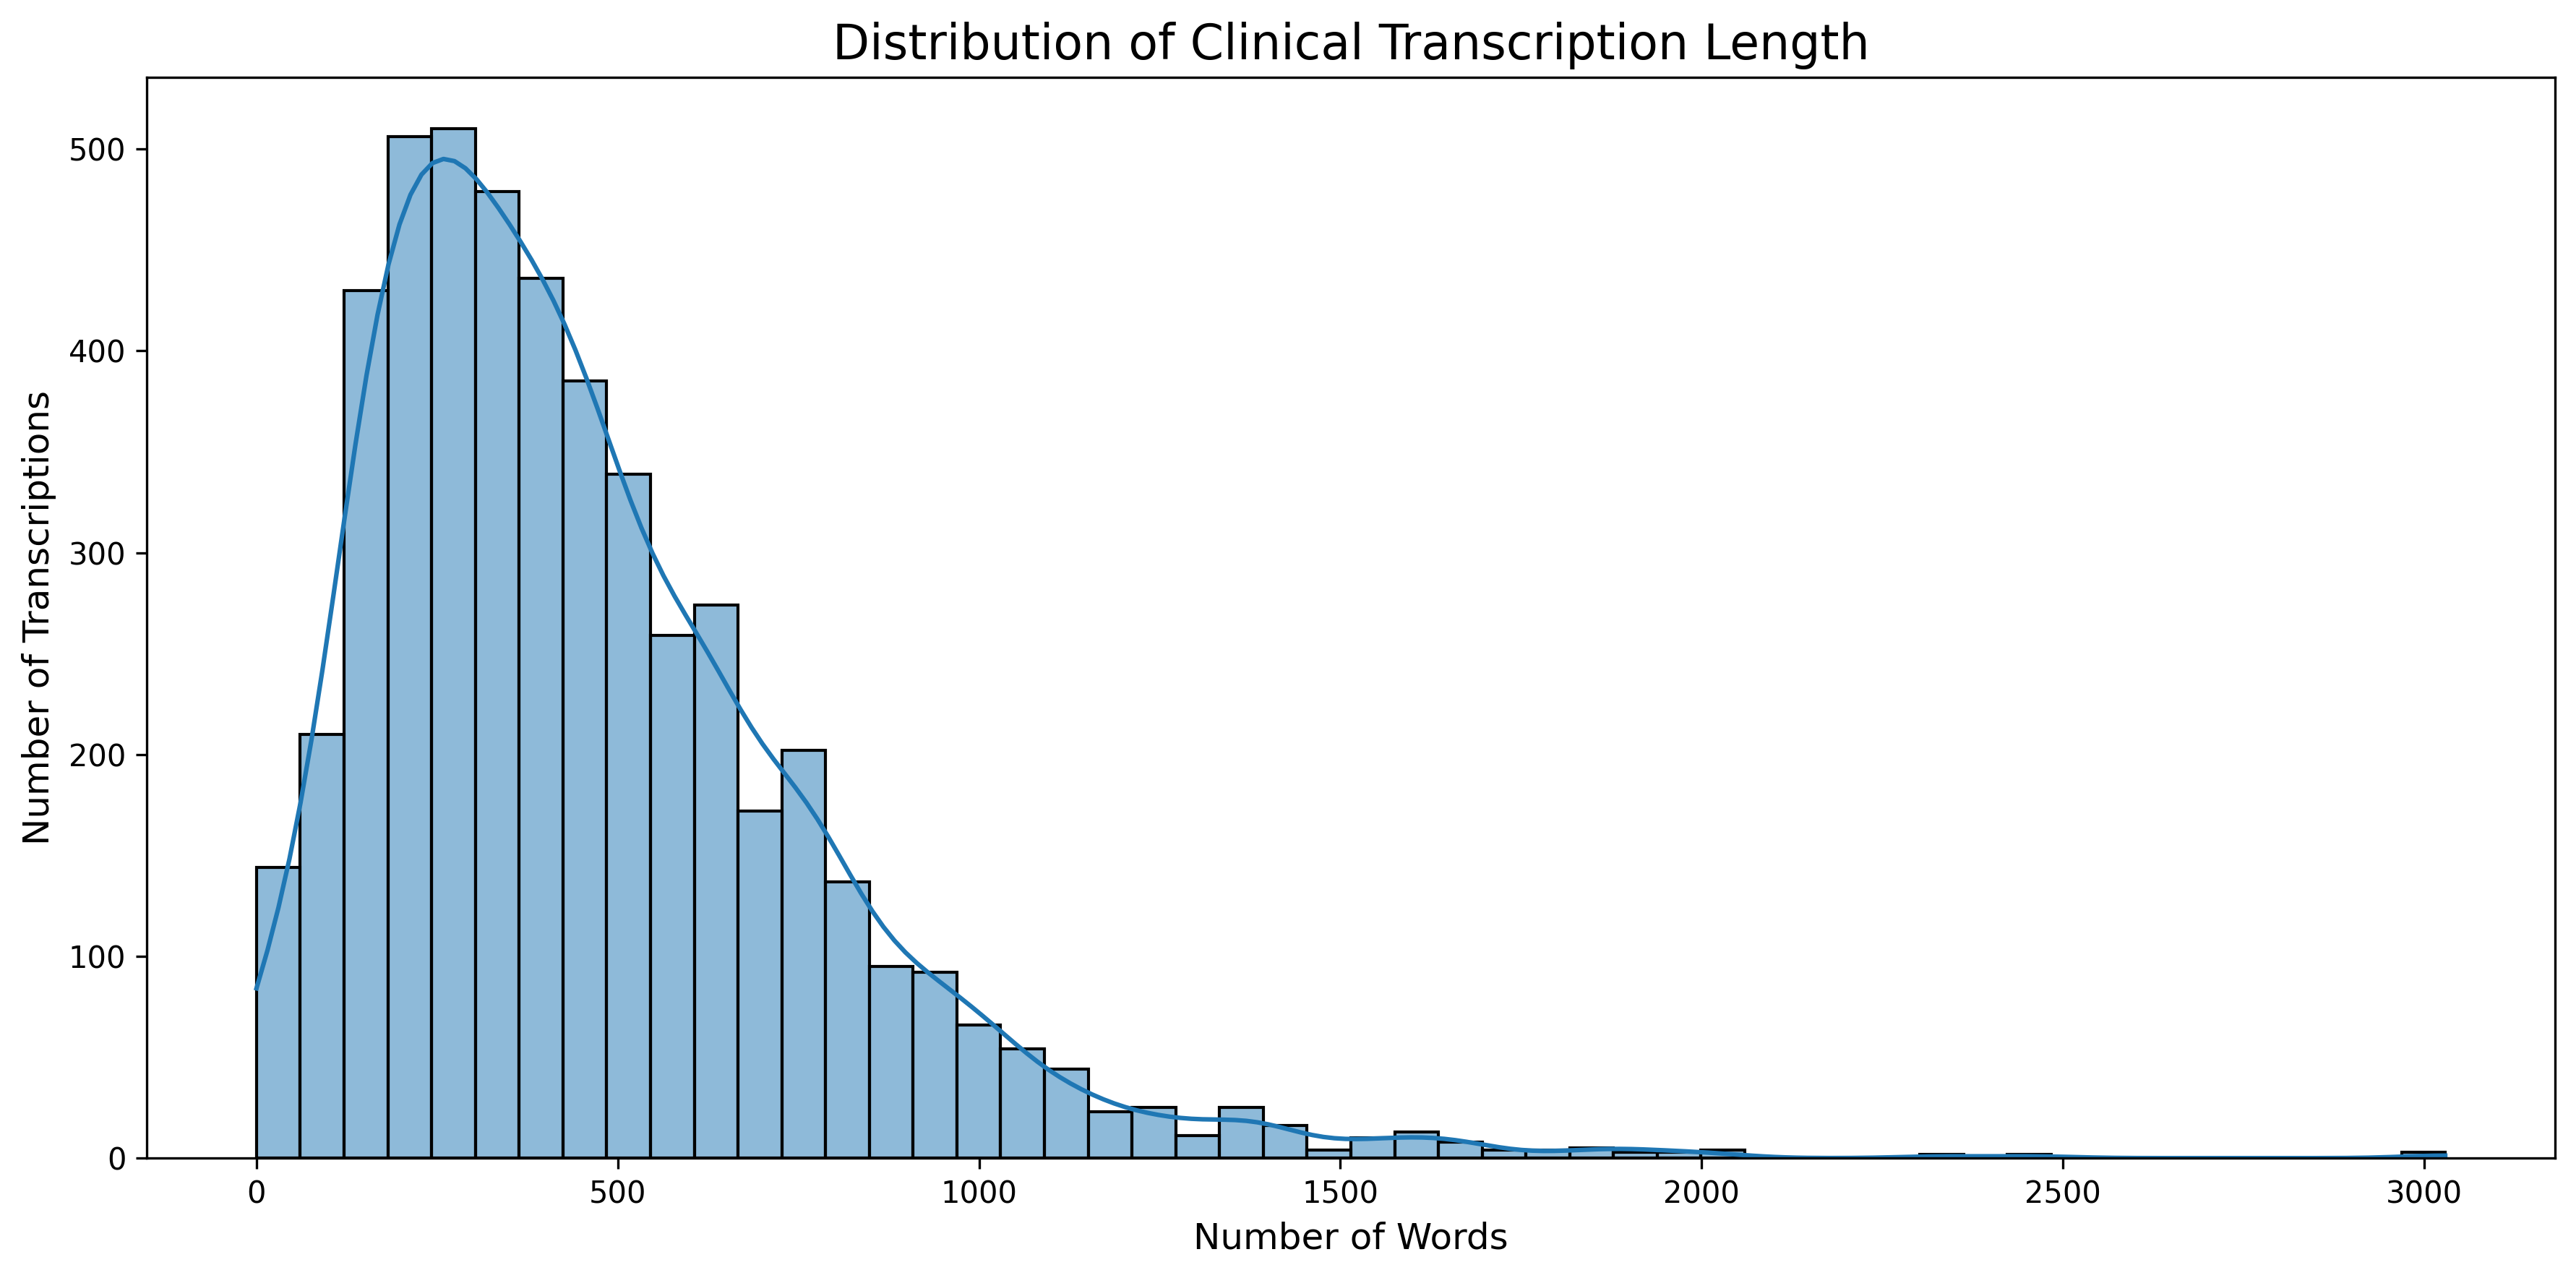
\includegraphics[width=0.82\textwidth,height=6.0cm,keepaspectratio]{EDA_Diagrams/04_transcription_length_distribution.png}
\caption{Distribution of Clinical Transcription Length}
\label{fig:eda_length_dist}
\end{figure}

\paragraph{Transcription Length Across Top Specialties}
Figure \ref{fig:eda_length_by_specialty} presents box plots comparing narrative word count distributions across the top 10 medical specialties. Specialties such as Radiology and Gastroenterology feature shorter median narrative lengths (~250 words), whereas Orthopedic, Surgery, and Consult - History and Phy. contain longer document narratives (median ~500 words) with multiple high-length outliers exceeding 1,500 to 2,500 words.

\begin{figure}[H]
\centering
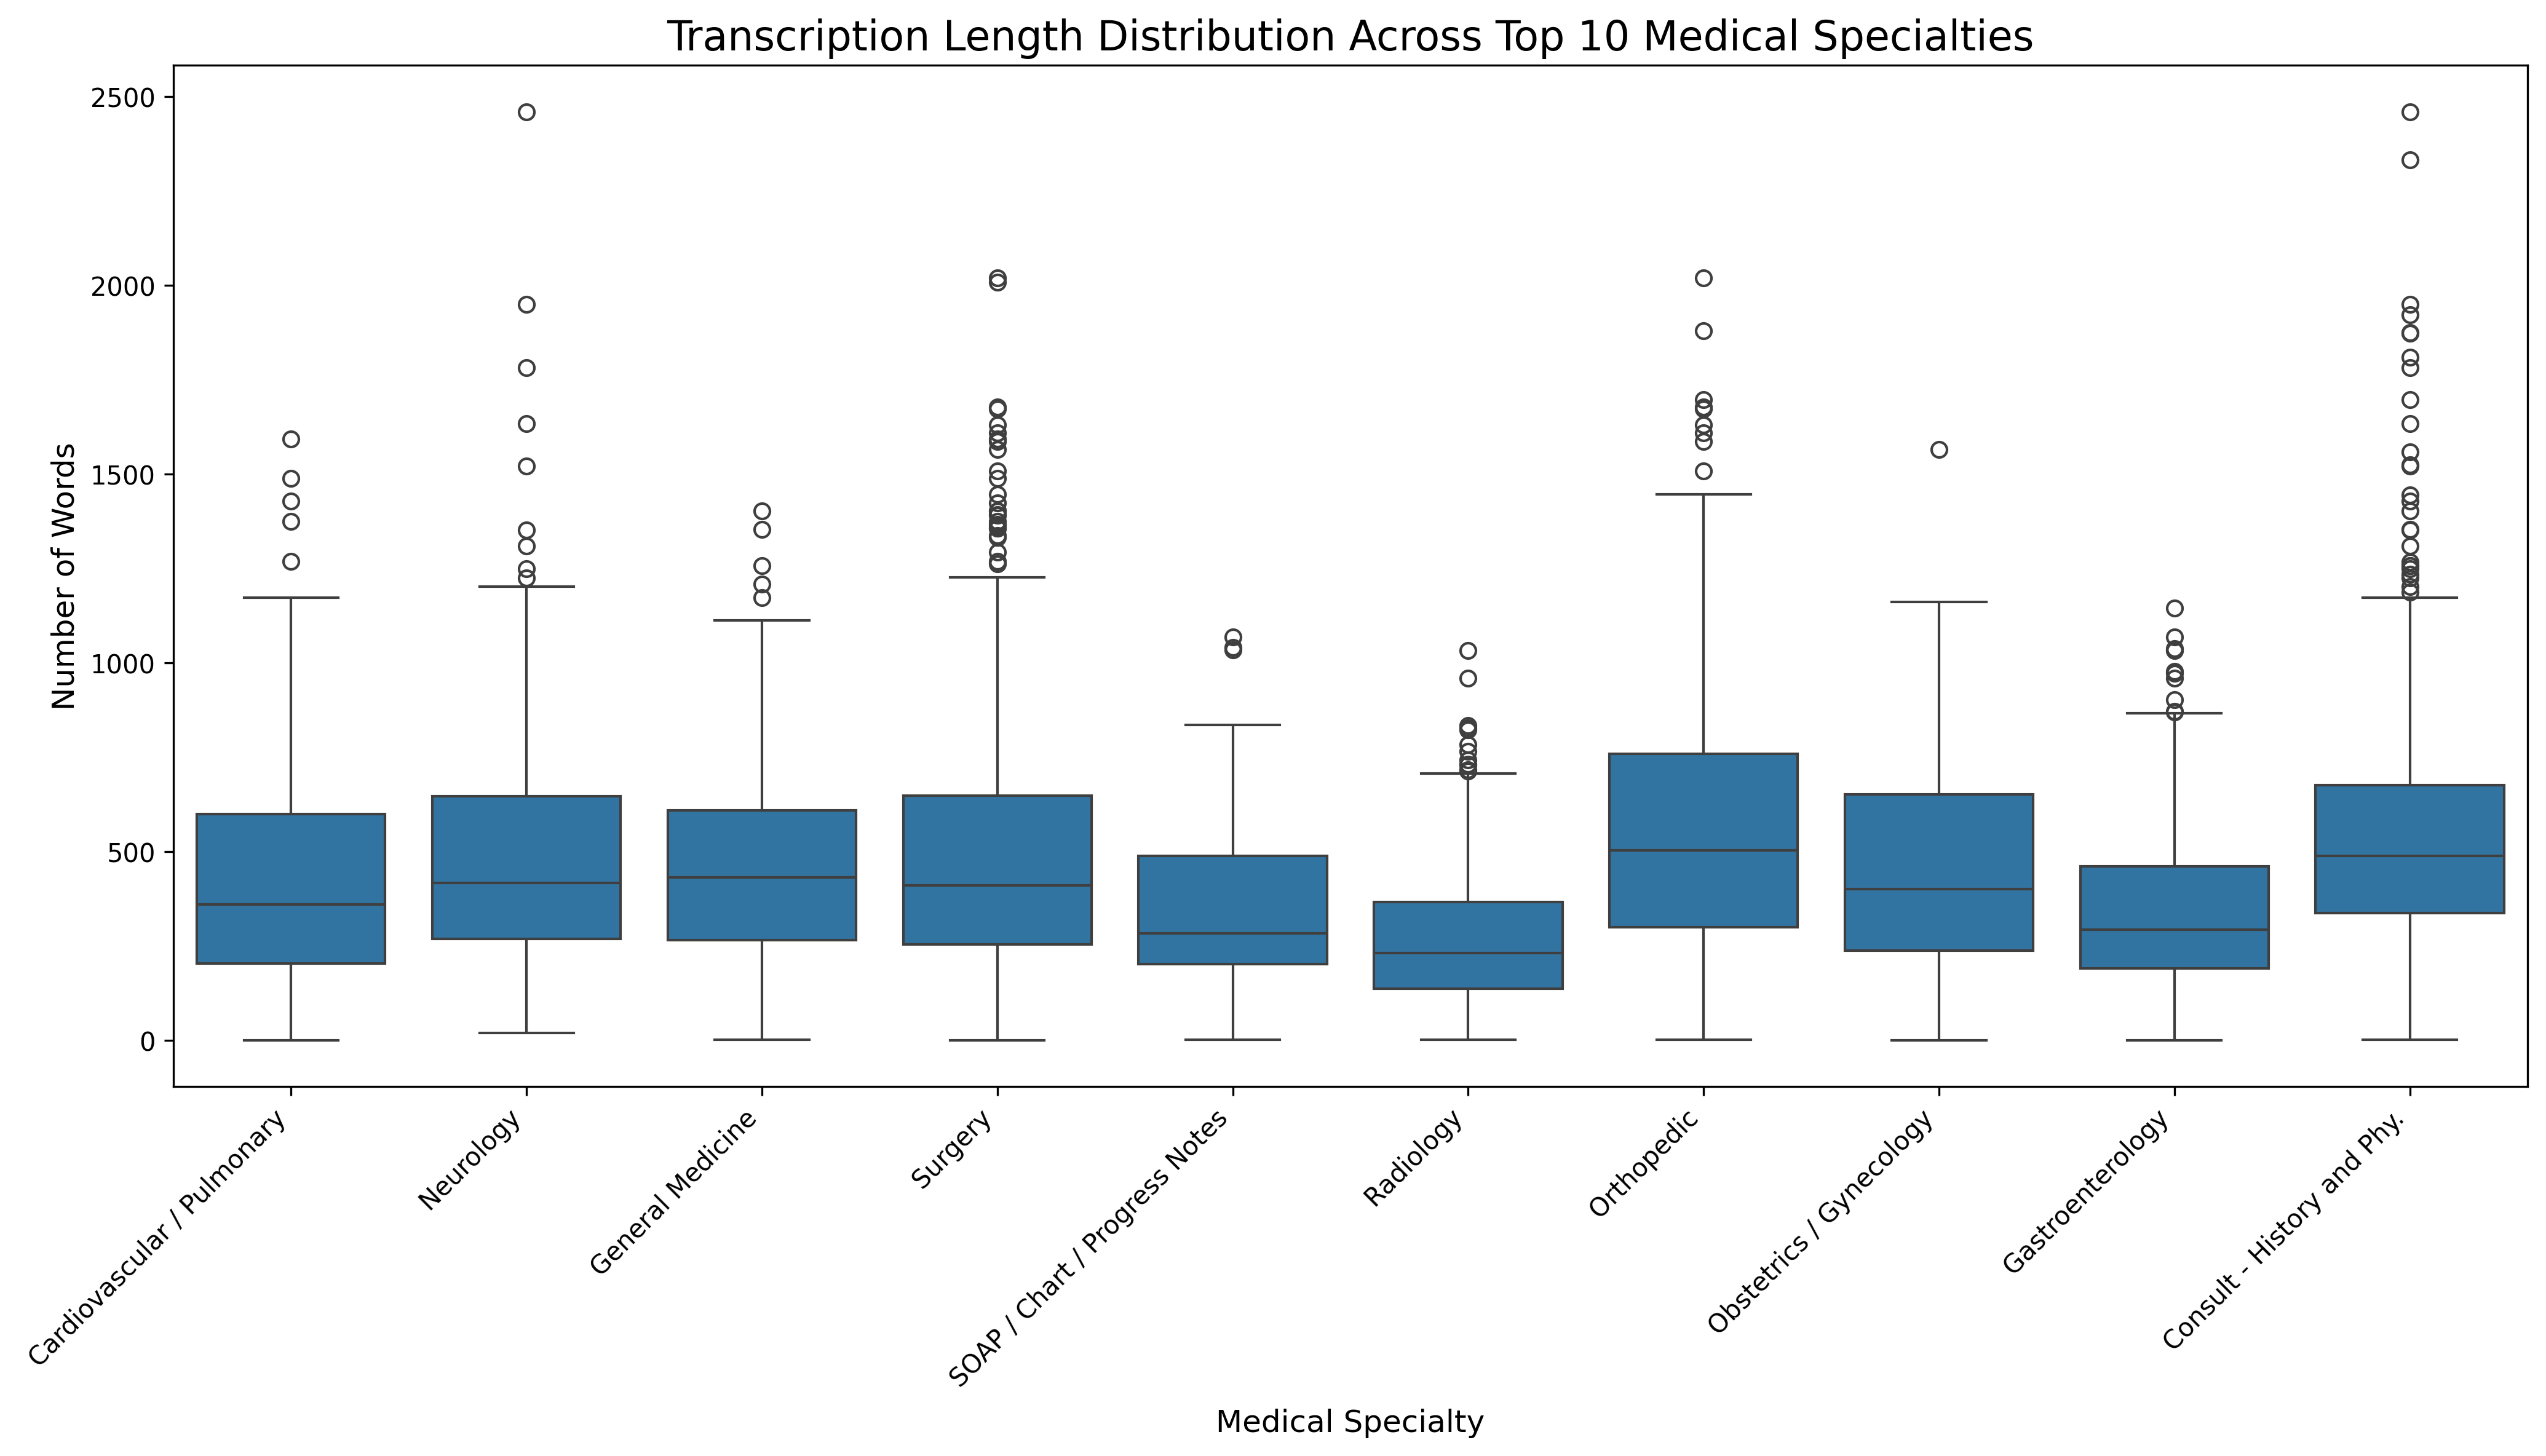
\includegraphics[width=0.82\textwidth,height=6.5cm,keepaspectratio]{EDA_Diagrams/05_transcription_length_by_specialty.png}
\caption{Transcription Length Distribution Across Top 10 Medical Specialties}
\label{fig:eda_length_by_specialty}
\end{figure}

\paragraph{Medical Word Cloud Visualization}
Figure \ref{fig:eda_wordcloud} displays a word cloud of the most frequent clinical terms extracted from the medical transcription corpus. High-frequency domain terms include "placed", "well", "used", "time", "patient", "incision", "removed", "normal", and "procedure", reflecting common clinical documentation vocabulary across specialties.

\begin{figure}[H]
\centering
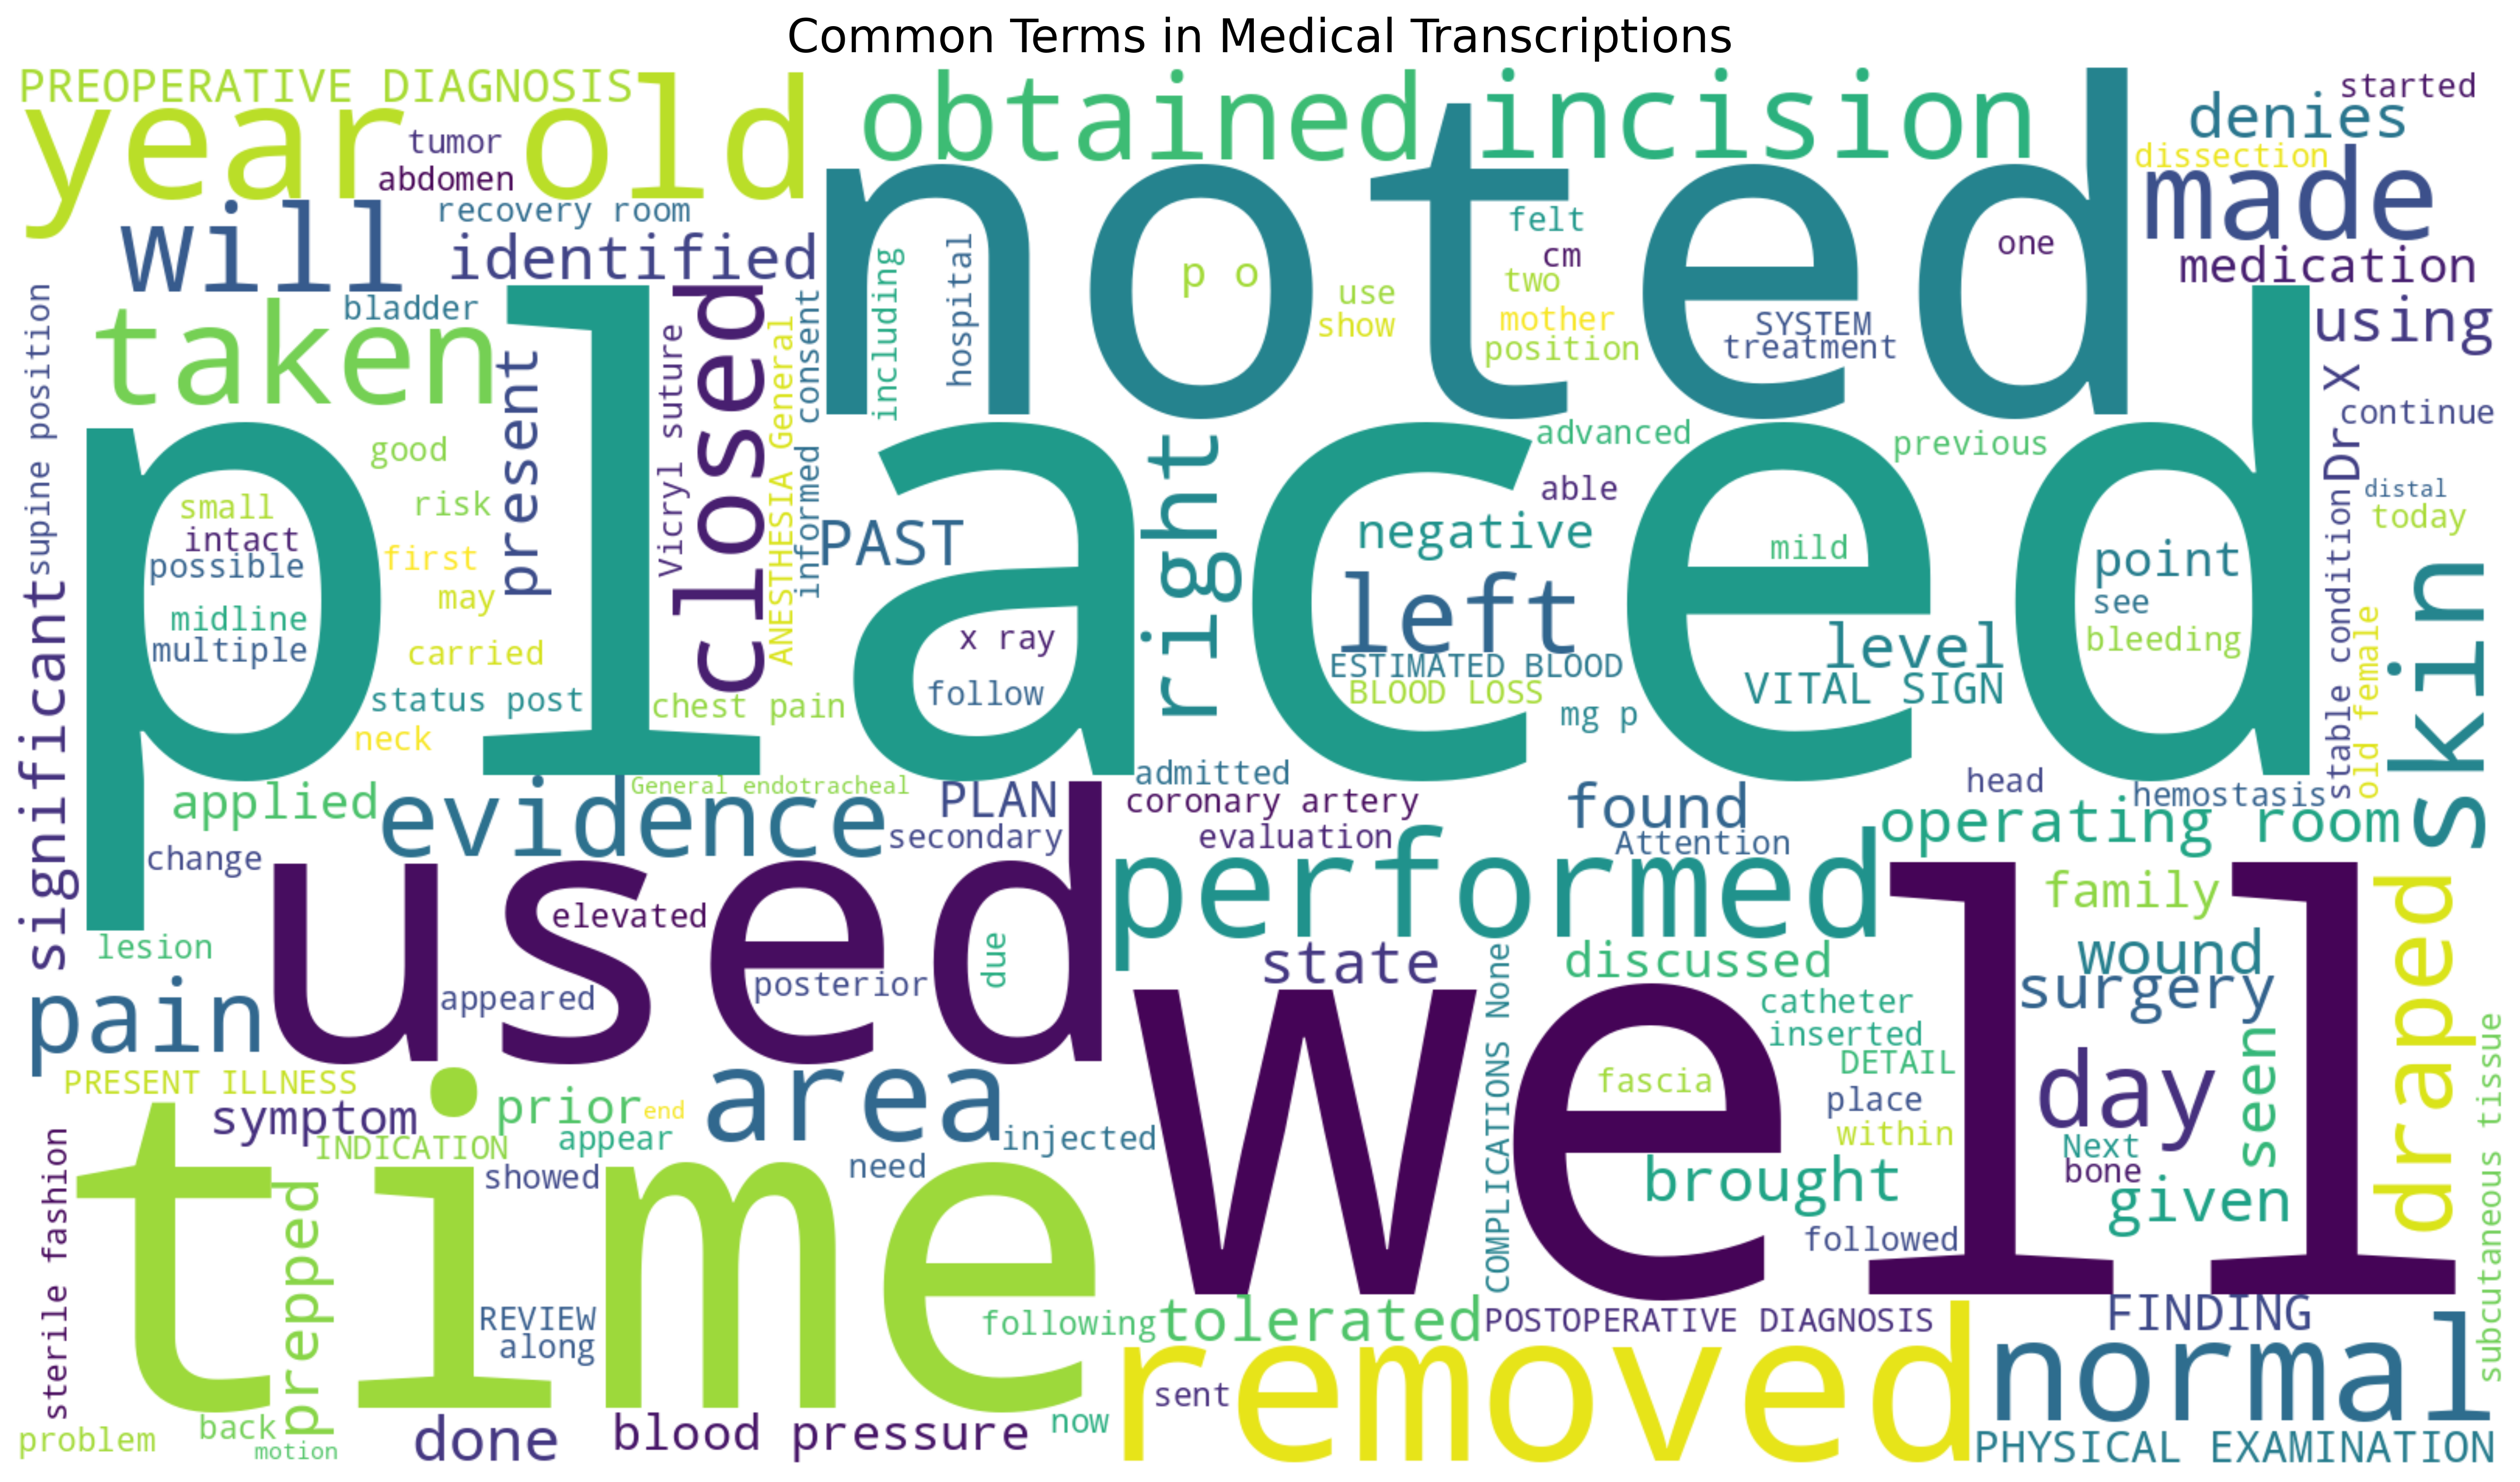
\includegraphics[width=0.82\textwidth,height=6.0cm,keepaspectratio]{EDA_Diagrams/06_medical_transcription_wordcloud.png}
\caption{Common Terms in Medical Transcriptions}
\label{fig:eda_wordcloud}
\end{figure}

The exploratory visualizations indicate that the clinical narratives exhibit distinct length characteristics, rich medical vocabulary, and severe class imbalance across specialties. These insights inform the text preprocessing, TF-IDF feature extraction, and stratified multi-model ensemble training strategies.

\clearpage

\subsection{DATA PREPROCESSING}

Data preprocessing is an essential stage in developing a machine learning model, as it transforms raw, unstructured clinical narratives into a structured and meaningful format suitable for mathematical modeling. In this project, the original dataset consisted of free-text clinical dictations containing clinical terminology, punctuation, formatting artifacts, and varying narrative lengths. The preprocessing stage included data cleaning, text normalization, analysis of feature variables, and examination of the target class distribution.

\subsubsection{DATA CLEANING}
Text preprocessing is essential in clinical NLP to remove noisy elements, normalize medical vocabulary, and transform raw narrative text into clean input suitable for mathematical vectorization. The cleaning pipeline executes eight sequential operations:

\begin{enumerate}
    \item \textit{Removing Missing Values}: Records containing empty or null \texttt{transcription} fields (33 records) are dropped from the dataset.
    \item \textit{Removing Duplicates}: Verification ensures no duplicate clinical reports exist in the corpus.
    \item \textit{Lowercasing}: All narrative text is converted to lowercase to standardize character representations.
    \item \textit{Removing Punctuation}: Commas, periods, semicolons, and special punctuation symbols are stripped.
    \item \textit{Removing Special Characters}: Numeric digits and non-alphanumeric symbols are removed.
    \item \textit{Tokenization}: Free-text narratives are segmented into individual word tokens.
    \item \textit{Stop-Word Removal}: Generic English stop-words are filtered out while preserving clinical vocabulary.
    \item \textit{Lemmatization}: Word tokens are mapped to their canonical base form using the WordNet Lemmatizer.
\end{enumerate}

Table \ref{tab:preprocessing_examples} provides concrete text transformation examples for each step.

\begin{table}[H]
\centering
\small
\setlength{\tabcolsep}{5pt}
\begin{tabularx}{\linewidth}{|>{\raggedright\arraybackslash}p{3.2cm}|>{\raggedright\arraybackslash}X|>{\raggedright\arraybackslash}X|}
\hline
\textbf{Preprocessing Step} & \textbf{Input Text Example} & \textbf{Processed Output Example} \\
\hline
Raw Input Text & "SUBJECTIVE: Patient suffers from acute chest pain!" & "SUBJECTIVE: Patient suffers from acute chest pain!" \\
\hline
1. Missing Values & Checked: Non-null text & Retained \\
\hline
2. Duplicates & Checked: Unique entry & Retained \\
\hline
3. Lowercasing & "SUBJECTIVE: Patient suffers..." & "subjective: patient suffers from acute chest pain!" \\
\hline
4. Punctuation & "subjective: patient suffers..." & "subjective patient suffers from acute chest pain" \\
\hline
5. Special Chars & "chest pain! 100\%" & "chest pain" \\
\hline
6. Tokenization & "patient suffers pain" & ['patient', 'suffers', 'pain'] \\
\hline
7. Stop-Words & ['patient', 'suffers', 'from', 'pain'] & ['patient', 'suffers', 'pain'] \\
\hline
8. Lemmatization & ['patient', 'suffers', 'pain'] & ['patient', 'suffer', 'pain'] \\
\hline
\end{tabularx}
\caption{Step-by-Step Clinical Text Preprocessing Examples}
\label{tab:preprocessing_examples}
\end{table}

\subsubsection{ANALYSIS OF FEATURE VARIABLES}
The \texttt{transcription} field is selected as the sole feature variable because it contains full clinical narratives describing patient symptoms, diagnostic findings, and surgical procedures. Metadata fields (\texttt{description}, \texttt{keywords}) are excluded due to high missingness. Unstructured clinical narratives are converted into high-dimensional numerical feature vectors using Term Frequency--Inverse Document Frequency (TF-IDF) vectorization, which extracts unigram and bigram tokens while applying sublinear frequency scaling and $L_2$ normalization.

\subsubsection{ANALYSIS OF CLASS VARIABLE}
The target variable \texttt{medical\_specialty} contains 40 distinct diagnostic categories. The class distribution exhibits severe imbalance, ranging from 1,103 reports in Surgery to only 2 reports in Autopsy and Executive Evaluation. To ensure fair multi-class evaluation, stratified train-test splitting (80:20) is utilized to preserve class proportions, and ensemble voting consensus is deployed to avoid model bias toward majority classes.

\clearpage

\subsection{ANALYSIS OF ALGORITHMS}

This project employs supervised machine learning algorithms to classify clinical transcription narratives into 40 distinct medical specialties. Multiple classification algorithms are considered to evaluate their effectiveness in distinguishing domain-specific clinical vocabulary based on extracted TF-IDF feature vectors. The proposed algorithms include Support Vector Machine (Linear SVM), Random Forest (RF), Logistic Regression (LR), and Multinomial Naive Bayes (MNB), integrated through a Voting Ensemble Classifier. These algorithms were chosen because they offer strong predictive performance in high-dimensional sparse text domains, provide architectural diversity, and execute efficiently on standard computing hardware without requiring specialized GPU accelerators.

\subsubsection{DETAILED STUDY REPORT OF THE PROPOSED ALGORITHMS}

The proposed system evaluates diverse machine learning estimators alongside statistical feature extraction to construct a robust diagnostic classification engine. Each algorithm offers distinct theoretical properties, mathematical formulations, and operational characteristics when applied to high-dimensional clinical text spaces.

\paragraph{1. Support Vector Machine (SVM)}

Support Vector Machine (SVM) is a robust supervised learning algorithm founded on statistical learning theory and structural risk minimization principles. It constructs an optimal decision boundary (hyperplane) in a high-dimensional feature space to separate target classes while maximizing the geometric margin between them. Linear SVM (Linear SVC) is exceptionally well suited for text categorization where sparse TF-IDF vectors offer natural linear separability.

\subparagraph{A. Theoretical Foundation and Optimization Model}
Given a training dataset $D = \{(x_1, y_1), (x_2, y_2), \dots, (x_N, y_N)\}$, where $x_i \in \mathbb{R}^d$ represents the sparse TF-IDF feature vector of $d$ vocabulary terms and $y_i \in \{1, 2, \dots, K\}$ denotes the target medical specialty ($K = 40$), the linear decision hyperplane is defined as:
\begin{equation}
w^T x + b = 0
\end{equation}
where $w \in \mathbb{R}^d$ is the weight vector normal to the hyperplane and $b \in \mathbb{R}$ is the bias scalar. To handle real-world clinical vocabulary noise and lexical overlap between specialties, a soft-margin optimization formulation is applied using non-negative slack variables $\xi_i \ge 0$:
\begin{equation}
\min_{w, b, \xi} \frac{1}{2} \|w\|^2 + C \sum_{i=1}^{N} \xi_i
\end{equation}
subject to the linear constraints:
\begin{equation}
y_{i, k}(w_k^T x_i + b_k) \ge 1 - \xi_i, \quad \xi_i \ge 0, \quad \forall i = 1, \dots, N
\end{equation}
where $C > 0$ is the regularization parameter controlling the trade-off between maximizing the geometric margin width ($\frac{2}{\|w\|}$) and minimizing training classification error.

\subparagraph{B. Dual Formulation and Multi-Class Decision Function}
By introducing Lagrange multipliers $\alpha_i \ge 0$, the primal optimization problem is transformed into its Wolfe dual representation:
\begin{equation}
\max_{\alpha} \sum_{i=1}^{N} \alpha_i - \frac{1}{2} \sum_{i=1}^{N} \sum_{j=1}^{N} \alpha_i \alpha_j y_i y_j K(x_i, x_j)
\end{equation}
subject to $0 \le \alpha_i \le C$ and $\sum_{i=1}^{N} \alpha_i y_i = 0$. For high-dimensional sparse text vectors, the Linear Kernel $K(x_i, x_j) = x_i^T x_j$ is utilized.

To support 40 medical specialties, a One-vs-Rest (OvR) strategy is implemented, training 40 independent binary classifiers. The decision function evaluating an incoming clinical transcription $x$ is:
\begin{equation}
f_k(x) = w_k^T x + b_k
\end{equation}
The predicted medical specialty $\hat{y}$ corresponds to the class with the maximum decision score:
\begin{equation}
\hat{y} = \arg\max_{k \in \{1, \dots, K\}} (w_k^T x + b_k)
\end{equation}

\subparagraph{C. Hyperparameter Tuning and Clinical Relevance}
The predictive performance of Linear SVM depends primarily on optimizing the regularization parameter $C$. Linear SVM excels in clinical transcription classification due to its immunity to high-dimensional overfitting, low memory footprint during inference, and reliance solely on critical support vectors along decision margins.

\begin{figure}[H]
\centering
\begin{tikzpicture}[node distance=0.24cm, auto, >=stealth',
    startstop/.style={rectangle, rounded corners=8pt, draw, fill=gray!12, text width=9em, text centered, minimum height=1.5em, font=\scriptsize\bfseries},
    process/.style={rectangle, draw, fill=blue!8, text width=14em, text centered, rounded corners=2pt, minimum height=1.5em, font=\scriptsize},
    decision/.style={diamond, draw, fill=yellow!12, text width=5.5em, text centered, inner sep=0pt, font=\scriptsize},
    branch/.style={rectangle, draw, fill=green!10, text width=6.5em, text centered, rounded corners=2pt, minimum height=1.5em, font=\scriptsize},
    arrow/.style={draw, -latex', semithick}]
    
    \node [startstop] (start) {START};
    \node [process, below=0.24cm of start] (p1) {Input Training TF-IDF Vectors};
    \node [process, below=0.24cm of p1] (p2) {Determine Decision Hyperplanes};
    \node [process, below=0.24cm of p2] (p3) {Calculate Margin ($\frac{2}{\|w\|}$)};
    \node [process, below=0.24cm of p3] (p4) {Identify Critical Support Vectors};
    \node [process, below=0.24cm of p4] (p5) {Optimize Hyperplane and Margin};
    \node [decision, below=0.28cm of p5] (dec1) {Converged?};
    \node [process, below=0.28cm of dec1] (p6) {Trained Multi-Class SVM Model};
    \node [process, below=0.24cm of p6] (p7) {Input New Clinical Transcription};
    \node [process, below=0.24cm of p7] (p8) {Compute Decision Values $f_k(x) = w_k^T x + b_k$};
    \node [process, below=0.24cm of p8] (p9) {Select Maximum Margin Class ($\arg\max$)};
    \node [branch, below=0.24cm of p9] (out) {Predicted Medical Specialty};
    \node [startstop, below=0.24cm of out] (end) {END};
    
    \path [arrow] (start) -- (p1);
    \path [arrow] (p1) -- (p2);
    \path [arrow] (p2) -- (p3);
    \path [arrow] (p3) -- (p4);
    \path [arrow] (p4) -- (p5);
    \path [arrow] (p5) -- (dec1);
    \path [arrow] (dec1.west) -- node[above, font=\tiny]{No} ++(-0.6cm,0) |- (p2.west);
    \path [arrow] (dec1.south) -- node[right, font=\tiny]{Yes} (p6);
    \path [arrow] (p6) -- (p7);
    \path [arrow] (p7) -- (p8);
    \path [arrow] (p8) -- (p9);
    \path [arrow] (p9) -- (out);
    \path [arrow] (out) -- (end);
\end{tikzpicture}
\caption{Activity Diagram of Support Vector Machine}
\label{fig:act_svm}
\end{figure}

\clearpage

\paragraph{2. Random Forest (RF)}

Random Forest is a high-performance ensemble learning algorithm based on decision tree aggregation. It constructs a multitude of uncorrelated decision trees during training and outputs the ensemble consensus. By combining Bootstrap Aggregation (Bagging) with random feature subspace selection, Random Forest mitigates variance without increasing prediction bias.

\subparagraph{A. Architectural Mechanics and Ensemble Formulation}
Given a training dataset of $N$ clinical transcription records, Random Forest generates $B$ bootstrap samples by sampling with replacement. For each bootstrap sample, an individual decision tree $T_b(x)$ is trained. At each split node of every tree, a random subset of $m = \sqrt{d}$ TF-IDF features is evaluated to identify the optimal split.

The final specialty class prediction for an input vector $x$ is derived through majority voting:
\begin{equation}
\hat{y} = \text{mode}(T_1(x), T_2(x), \dots, T_B(x))
\end{equation}
Alternatively, posterior class probabilities are computed as the average over all $B$ decision trees:
\begin{equation}
P(y = k \mid x) = \frac{1}{B} \sum_{b=1}^{B} P_b(y = k \mid x)
\end{equation}

\subparagraph{B. Node Splitting Criteria and Impurity Measures}
Decision tree node splits are evaluated using impurity metrics such as Gini Impurity or Information Gain (Entropy).
\begin{itemize}
    \item \textbf{Gini Impurity ($G$)}:
    \begin{equation}
    G = 1 - \sum_{k=1}^{K} p_k^2
    \end{equation}
    where $p_k$ represents the proportion of instances belonging to specialty class $k \in \{1, \dots, 40\}$ at a given node.
    \item \textbf{Entropy ($H$) and Information Gain ($IG$)}:
    \begin{equation}
    H(S) = -\sum_{k=1}^{K} p_k \log_2(p_k)
    \end{equation}
    \begin{equation}
    IG(S, A) = H(S) - \sum_{v \in \text{Values}(A)} \frac{|S_v|}{|S|} H(S_v)
    \end{equation}
\end{itemize}

\subparagraph{C. Feature Importance Analysis and Clinical Interpretability}
A major benefit of Random Forest is its capacity to quantify feature importance using Mean Decrease in Impurity (MDI). The importance index $I(A_j)$ of TF-IDF feature $A_j$ across all $B$ decision trees is computed as:
\begin{equation}
I(A_j) = \frac{1}{B} \sum_{b=1}^{B} \sum_{n \in N_b(A_j)} \Delta G(n)
\end{equation}
where $\Delta G(n)$ is the Gini impurity reduction achieved at node $n$ by splitting on feature $A_j$. In clinical NLP, this enables identification and ranking of the most discriminative medical keywords for each specialty.

\subparagraph{D. Hyperparameter Optimization}
The primary hyperparameters tuned for Random Forest include:
\begin{itemize}
    \item \texttt{n\_estimators} ($B$): Number of decision trees (typically 100 to 300).
    \item \texttt{max\_depth}: Maximum depth of decision trees to prevent single-tree memorization.
    \item \texttt{min\_samples\_split}: Minimum samples required to split an internal node.
    \item \texttt{min\_samples\_leaf}: Minimum samples required at a terminal leaf node.
\end{itemize}
Random Forest captures complex non-linear keyword interactions that linear models may overlook, adding structural diversity to the ensemble.

\begin{figure}[H]
\centering
\begin{tikzpicture}[node distance=0.24cm, auto, >=stealth',
    startstop/.style={rectangle, rounded corners=8pt, draw, fill=gray!12, text width=9em, text centered, minimum height=1.5em, font=\scriptsize\bfseries},
    process/.style={rectangle, draw, fill=blue!8, text width=14em, text centered, rounded corners=2pt, minimum height=1.5em, font=\scriptsize},
    decision/.style={diamond, draw, fill=yellow!12, text width=5.5em, text centered, inner sep=0pt, font=\scriptsize},
    branch/.style={rectangle, draw, fill=green!10, text width=6.5em, text centered, rounded corners=2pt, minimum height=1.5em, font=\scriptsize},
    arrow/.style={draw, -latex', semithick}]
    
    \node [startstop] (start) {START};
    \node [process, below=0.24cm of start] (p1) {Input Training TF-IDF Vectors};
    \node [process, below=0.24cm of p1] (p2) {Generate Bootstrap Sample};
    \node [process, below=0.24cm of p2] (p3) {Select Random Feature Subset ($m = \sqrt{d}$)};
    \node [process, below=0.24cm of p3] (p4) {Build Decision Tree via Gini Split};
    \node [decision, below=0.28cm of p4] (dec1) {More Trees?};
    \node [process, below=0.28cm of dec1] (p5) {Forest of Decision Trees Completed};
    \node [process, below=0.24cm of p5] (p6) {Input New Clinical Transcription};
    \node [process, below=0.24cm of p6] (p7) {Obtain Predictions from Each Tree};
    \node [process, below=0.24cm of p7] (p8) {Apply Probability Averaging};
    \node [branch, below=0.24cm of p8] (out) {Predicted Medical Specialty};
    \node [startstop, below=0.24cm of out] (end) {END};
    
    \path [arrow] (start) -- (p1);
    \path [arrow] (p1) -- (p2);
    \path [arrow] (p2) -- (p3);
    \path [arrow] (p3) -- (p4);
    \path [arrow] (p4) -- (dec1);
    \path [arrow] (dec1.west) -- node[above, font=\tiny]{Yes} ++(-0.6cm,0) |- (p2.west);
    \path [arrow] (dec1.south) -- node[right, font=\tiny]{No} (p5);
    \path [arrow] (p5) -- (p6);
    \path [arrow] (p6) -- (p7);
    \path [arrow] (p7) -- (p8);
    \path [arrow] (p8) -- (out);
    \path [arrow] (out) -- (end);
\end{tikzpicture}
\caption{Activity Diagram of Random Forest}
\label{fig:act_rf}
\end{figure}

\clearpage

\paragraph{3. Logistic Regression (LR)}

Logistic Regression is a foundational statistical learning algorithm for classification problems. Belonging to the family of Generalized Linear Models (GLMs), it is extended to multi-class classification using the multinomial Softmax formulation, modeling posterior probabilities directly.

\subparagraph{A. Probabilistic Model and Multinomial Softmax Transformation}
For an input TF-IDF vector $x \in \mathbb{R}^d$ and $K = 40$ medical specialty classes, the algorithm computes linear logit scores $z_k = w_k^T x + b_k$. The posterior probability that transcription $x$ belongs to specialty $k$ is given by the Softmax function:
\begin{equation}
P(y = k \mid x) = \frac{\exp(w_k^T x + b_k)}{\sum_{j=1}^{K} \exp(w_j^T x + b_j)}
\end{equation}
where $w_k \in \mathbb{R}^d$ is the weight vector associated with specialty $k$ and $b_k \in \mathbb{R}$ is the class-specific bias term.

\subparagraph{B. Maximum Likelihood Estimation and Loss Function}
Model parameter estimation is performed by minimizing the Categorical Cross-Entropy (Negative Log-Likelihood) loss function over $N$ training samples, augmented with an $L_2$ Ridge penalty:
\begin{equation}
J(W, b) = -\frac{1}{N} \sum_{i=1}^{N} \sum_{k=1}^{K} \mathbb{I}(y_i = k) \ln P(y_i = k \mid x_i) + \frac{\lambda}{2} \sum_{k=1}^{K} \|w_k\|_2^2
\end{equation}
where $\mathbb{I}(\cdot)$ is the indicator function, and $\lambda > 0$ controls the regularisation strength to prevent coefficient explosion on sparse text inputs. Parameters are optimized via gradient descent algorithms:
\begin{equation}
w_k^{(t+1)} = w_k^{(t)} - \alpha \nabla_{w_k} J(W, b)
\end{equation}

\subparagraph{C. Clinical Relevance and Interpretability}
Logistic Regression serves as an essential baseline model due to its high interpretability. The exponentiated weight coefficients $\exp(w_{k, j})$ represent odds ratios for clinical terms, providing quantitative insight into which medical keywords escalate the probability of assigning a transcription to a specific specialty.

\begin{figure}[H]
\centering
\begin{tikzpicture}[node distance=0.24cm, auto, >=stealth',
    startstop/.style={rectangle, rounded corners=8pt, draw, fill=gray!12, text width=9em, text centered, minimum height=1.5em, font=\scriptsize\bfseries},
    process/.style={rectangle, draw, fill=blue!8, text width=14em, text centered, rounded corners=2pt, minimum height=1.5em, font=\scriptsize},
    decision/.style={diamond, draw, fill=yellow!12, text width=5.5em, text centered, inner sep=0pt, font=\scriptsize},
    branch/.style={rectangle, draw, fill=green!10, text width=6.5em, text centered, rounded corners=2pt, minimum height=1.5em, font=\scriptsize},
    arrow/.style={draw, -latex', semithick}]
    
    \node [startstop] (start) {START};
    \node [process, below=0.24cm of start] (p1) {Input Training TF-IDF Vectors};
    \node [process, below=0.24cm of p1] (p2) {Initialize Weights and Biases};
    \node [process, below=0.24cm of p2] (p3) {Calculate Linear Scores $z_k = w_k^T x + b_k$};
    \node [process, below=0.24cm of p3] (p4) {Apply Softmax Activation Function};
    \node [process, below=0.24cm of p4] (p5) {Calculate Cross-Entropy Loss};
    \node [process, below=0.24cm of p5] (p6) {Update Weights via Gradient Descent};
    \node [decision, below=0.28cm of p6] (dec1) {Converged?};
    \node [process, below=0.28cm of dec1] (p7) {Trained Logistic Regression Model};
    \node [process, below=0.24cm of p7] (p8) {Input New Clinical Transcription};
    \node [process, below=0.24cm of p8] (p9) {Calculate Class Probabilities $P(y=k|x)$};
    \node [process, below=0.24cm of p9] (p10) {Select Highest Probability Class};
    \node [branch, below=0.24cm of p10] (out) {Predicted Medical Specialty};
    \node [startstop, below=0.24cm of out] (end) {END};
    
    \path [arrow] (start) -- (p1);
    \path [arrow] (p1) -- (p2);
    \path [arrow] (p2) -- (p3);
    \path [arrow] (p3) -- (p4);
    \path [arrow] (p4) -- (p5);
    \path [arrow] (p5) -- (p6);
    \path [arrow] (p6) -- (dec1);
    \path [arrow] (dec1.west) -- node[above, font=\tiny]{No} ++(-0.6cm,0) |- (p3.west);
    \path [arrow] (dec1.south) -- node[right, font=\tiny]{Yes} (p7);
    \path [arrow] (p7) -- (p8);
    \path [arrow] (p8) -- (p9);
    \path [arrow] (p9) -- (p10);
    \path [arrow] (p10) -- (out);
    \path [arrow] (out) -- (end);
\end{tikzpicture}
\caption{Activity Diagram of Logistic Regression}
\label{fig:act_lr}
\end{figure}

\clearpage

\paragraph{4. Multinomial Naive Bayes (MNB)}

Multinomial Naive Bayes is a specialized probabilistic classification algorithm rooted in Bayes' Theorem, specifically formulated for discrete word counts and term frequency distributions in document categorization tasks.

\subparagraph{A. Probabilistic Foundation and Bayes' Theorem}
The algorithm computes the posterior probability of clinical transcription $x = (x_1, \dots, x_m)$ belonging to medical specialty class $c$ using Bayes' rule alongside the assumption of conditional feature independence given the class label:
\begin{equation}
P(c \mid x) \propto P(c) \prod_{i=1}^{m} P(x_i \mid c)
\end{equation}
where $P(c)$ is the prior probability of specialty $c$ (derived from training class proportions) and $P(x_i \mid c)$ is the class-conditional feature likelihood.

\subparagraph{B. Feature Likelihood and Laplace Smoothing}
To prevent zero-probability penalties for clinical terms absent in the training split of a specific specialty, Laplace (additive) smoothing is applied:
\begin{equation}
P(x_i \mid c) = \frac{N_{ci} + \alpha}{N_c + \alpha |V|}
\end{equation}
where $N_{ci}$ is the cumulative occurrence count of term $x_i$ in specialty class $c$, $N_c$ is the total token count across all records in class $c$, $|V|$ is the vocabulary size, and $\alpha = 1.0$ is the smoothing hyperparameter.

\subparagraph{C. Computational Efficiency and Role in Medical Text Classification}
Multinomial Naive Bayes executes in linear time with minimal memory overhead. It functions reliably on smaller clinical training subsets, providing an efficient baseline that contributes probabilistic diversity to the ensemble.

\begin{figure}[H]
\centering
\begin{tikzpicture}[node distance=0.24cm, auto, >=stealth',
    startstop/.style={rectangle, rounded corners=8pt, draw, fill=gray!12, text width=9em, text centered, minimum height=1.5em, font=\scriptsize\bfseries},
    process/.style={rectangle, draw, fill=blue!8, text width=14em, text centered, rounded corners=2pt, minimum height=1.5em, font=\scriptsize},
    branch/.style={rectangle, draw, fill=green!10, text width=6.5em, text centered, rounded corners=2pt, minimum height=1.5em, font=\scriptsize},
    arrow/.style={draw, -latex', semithick}]
    
    \node [startstop] (start) {START};
    \node [process, below=0.24cm of start] (p1) {Input Training TF-IDF Vectors};
    \node [process, below=0.24cm of p1] (p2) {Calculate Prior Probability $P(c)$};
    \node [process, below=0.24cm of p2] (p3) {Compute Term Frequency per Class};
    \node [process, below=0.24cm of p3] (p4) {Apply Additive Laplace Smoothing ($\alpha=1$)};
    \node [process, below=0.24cm of p4] (p5) {Trained Naive Bayes Model};
    \node [process, below=0.24cm of p5] (p6) {Input New Clinical Transcription};
    \node [process, below=0.24cm of p6] (p7) {Apply Bayes' Theorem for Posterior Prob.};
    \node [process, below=0.24cm of p7] (p8) {Select Maximum Probability Class};
    \node [branch, below=0.24cm of p8] (out) {Predicted Medical Specialty};
    \node [startstop, below=0.24cm of out] (end) {END};
    
    \path [arrow] (start) -- (p1);
    \path [arrow] (p1) -- (p2);
    \path [arrow] (p2) -- (p3);
    \path [arrow] (p3) -- (p4);
    \path [arrow] (p4) -- (p5);
    \path [arrow] (p5) -- (p6);
    \path [arrow] (p6) -- (p7);
    \path [arrow] (p7) -- (p8);
    \path [arrow] (p8) -- (out);
    \path [arrow] (out) -- (end);
\end{tikzpicture}
\caption{Activity Diagram of Multinomial Naive Bayes}
\label{fig:act_mnb}
\end{figure}

\clearpage

\paragraph{5. TF-IDF Feature Vectorizer}

Term Frequency--Inverse Document Frequency (TF-IDF) is a statistical vectorization technique that converts unstructured clinical text narratives into high-dimensional numerical feature vectors. In our proposed medical specialty classification system, TF-IDF operates as the core feature engineering component.

\subparagraph{A. Statistical Foundation and Mathematical Formulation}
The vectorization process evaluates the relative importance of each term $t$ within a specific document $d$ against the entire clinical corpus $D$. Term Frequency, denoted as $\text{TF}(t, d)$, measures word occurrences scaled sublinearly:
\begin{equation}
\text{TF}(t, d) = 1 + \log(f_{t, d}) \quad (\text{if } f_{t, d} > 0)
\end{equation}
Inverse Document Frequency, denoted as $\text{IDF}(t, D)$, computes the logarithmic inverse ratio:
\begin{equation}
\text{IDF}(t, D) = \log\left(\frac{1 + |D|}{1 + |\{d \in D : t \in d\}|}\right) + 1
\end{equation}
The composite TF-IDF weight is:
\begin{equation}
\text{TF-IDF}(t, d, D) = \text{TF}(t, d) \times \text{IDF}(t, D)
\end{equation}
To ensure comparability across documents of varying lengths, Euclidean $L_2$ normalization is applied:
\begin{equation}
v_{\text{norm}} = \frac{v}{\|v\|_2} = \frac{v}{\sqrt{\sum_i v_i^2}}
\end{equation}

\subparagraph{B. N-Gram Extraction and Sparsity Optimization}
The vectorizer extracts unigrams and bigrams, capturing both isolated medical terms (e.g., "appendectomy") and multi-word phrases (e.g., "coronary artery"). A minimum document frequency threshold filters out rare typos, yielding a normalized, highly efficient sparse matrix.

\subparagraph{C. Clinical Term Weighting and Down-Weighting Common Words}
Through this formulation, terms appearing across almost all reports receive low weights, whereas specialty-specific diagnostic vocabulary receives high discriminative weights.

\begin{figure}[H]
\centering
\begin{tikzpicture}[node distance=0.24cm, auto, >=stealth',
    startstop/.style={rectangle, rounded corners=8pt, draw, fill=gray!12, text width=9em, text centered, minimum height=1.5em, font=\scriptsize\bfseries},
    process/.style={rectangle, draw, fill=blue!8, text width=14em, text centered, rounded corners=2pt, minimum height=1.5em, font=\scriptsize},
    arrow/.style={draw, -latex', semithick}]
    
    \node [startstop] (start) {START};
    \node [process, below=0.24cm of start] (p1) {Input Cleaned Text Narratives};
    \node [process, below=0.24cm of p1] (p2) {Tokenize \& Generate N-Grams};
    \node [process, below=0.24cm of p2] (p3) {Compute Term Frequency ($\text{TF}$)};
    \node [process, below=0.24cm of p3] (p4) {Compute Inverse Doc Frequency ($\text{IDF}$)};
    \node [process, below=0.24cm of p4] (p5) {Calculate Composite Score ($\text{TF} \times \text{IDF}$)};
    \node [process, below=0.24cm of p5] (p6) {Apply Euclidean $L_2$ Normalization};
    \node [process, below=0.24cm of p6] (p7) {Construct Sparse Feature Matrix};
    \node [startstop, below=0.24cm of p7] (end) {END};
    
    \path [arrow] (start) -- (p1);
    \path [arrow] (p1) -- (p2);
    \path [arrow] (p2) -- (p3);
    \path [arrow] (p3) -- (p4);
    \path [arrow] (p4) -- (p5);
    \path [arrow] (p5) -- (p6);
    \path [arrow] (p6) -- (p7);
    \path [arrow] (p7) -- (end);
\end{tikzpicture}
\caption{Activity Diagram of TF-IDF Feature Vectorizer}
\label{fig:act_tfidf}
\end{figure}

\clearpage

\paragraph{6. Voting Ensemble Classifier}

The Voting Ensemble Classifier is the final meta-classification mechanism in the proposed system. Rather than relying on a single learning algorithm that may exhibit inductive biases across imbalanced specialties, the ensemble combines predictions from diverse candidate models (Logistic Regression, Linear SVM, Random Forest, and Multinomial Naive Bayes) to generate a consensus decision.

\subparagraph{A. Ensemble Mechanics and Soft-Voting Aggregation}
In the soft-voting configuration, each base classifier $m \in \{1, \dots, M\}$ generates a calibrated class probability distribution $P_m(y = k \mid x)$ indicating the likelihood that a given clinical transcription $x$ belongs to specialty $k$. The ensemble computes the arithmetic mean of these posterior probabilities across all $M$ estimators:
\begin{equation}
P_{\text{ensemble}}(y = k \mid x) = \frac{1}{M} \sum_{m=1}^{M} P_m(y = k \mid x)
\end{equation}

\subparagraph{B. Final Multi-Class Specialty Prediction}
The final predicted medical specialty $\hat{y}$ is selected as the category that maximizes the aggregated ensemble probability:
\begin{equation}
\hat{y} = \arg\max_{k \in \{1, \dots, K\}} P_{\text{ensemble}}(y = k \mid x)
\end{equation}

\subparagraph{C. Variance Reduction and Synergy of Diverse Estimators}
By integrating linear probabilistic modeling (Logistic Regression), maximum-margin geometric boundaries (Linear SVM), non-linear decision trees (Random Forest), and conditional frequency modeling (Multinomial Naive Bayes), the ensemble offsets the individual weaknesses of each classifier, reduces predictive variance, and improves overall classification stability across all 40 medical specialties.

\begin{figure}[H]
\centering
\begin{tikzpicture}[node distance=0.4cm and 0.2cm, auto, >=stealth',
    startstop/.style={rectangle, rounded corners=8pt, draw, fill=gray!12, text width=9em, text centered, minimum height=1.5em, font=\scriptsize\bfseries},
    process/.style={rectangle, draw, fill=green!10, text width=15em, text centered, rounded corners=2pt, minimum height=1.6em, font=\scriptsize},
    smallbox/.style={rectangle, draw, fill=blue!10, text width=5.6em, text centered, rounded corners=2pt, minimum height=2.2em, font=\scriptsize},
    branch/.style={rectangle, draw, fill=green!10, text width=7em, text centered, rounded corners=2pt, minimum height=1.5em, font=\scriptsize},
    arrow/.style={draw, -latex', semithick}]
    
    \node [startstop] (start) {START};
    \node [process, below=0.3cm of start] (input) {TF-IDF Feature Vector Input};
    
    \node [smallbox, below left=0.6cm and 1.8cm of input] (lr) {Logistic\\Regression};
    \node [smallbox, below left=0.6cm and 0.15cm of input] (svm) {Linear\\SVC / SVM};
    \node [smallbox, below right=0.6cm and 0.15cm of input] (rf) {Random\\Forest};
    \node [smallbox, below right=0.6cm and 1.8cm of input] (nb) {Multinomial\\Naive Bayes};
    
    \node [process, below=1.8cm of input] (collect) {Collect Predictions from All Classifiers};
    \node [process, below=0.3cm of collect] (vote) {Apply Soft-Voting Aggregation Strategy};
    \node [process, below=0.3cm of vote] (select) {Select Final Predicted Class ($\arg\max$)};
    \node [branch, below=0.3cm of select] (output) {Predicted Medical Specialty};
    \node [startstop, below=0.3cm of output] (end) {END};
    
    \path [arrow] (start) -- (input);
    \path [arrow] (input) -| (lr.north);
    \path [arrow] (input) -| (svm.north);
    \path [arrow] (input) -| (rf.north);
    \path [arrow] (input) -| (nb.north);
    
    \path [arrow] (lr.south) |- (collect);
    \path [arrow] (svm.south) |- (collect);
    \path [arrow] (rf.south) |- (collect);
    \path [arrow] (nb.south) |- (collect);
    
    \path [arrow] (collect) -- (vote);
    \path [arrow] (vote) -- (select);
    \path [arrow] (select) -- (output);
    \path [arrow] (output) -- (end);
\end{tikzpicture}
\caption{Activity Diagram of Voting Ensemble Classifier}
\label{fig:act_ensemble}
\end{figure}

\clearpage

\paragraph{Working of the Proposed Algorithms}
The proposed machine learning classification framework executes through the following nine sequential steps:
\begin{enumerate}
    \item \textbf{Dataset Ingestion}: Loading the raw Kaggle MTSamples dataset containing 4,999 clinical records across 40 medical specialties.
    \item \textbf{Data Cleaning}: Auditing and removing records with missing clinical transcriptions (33 null records), handling missing keywords (1,068 records), and standardizing text to lower case.
    \item \textbf{Text Preprocessing}: Eliminating punctuation marks, digits, symbols, and domain stop-words, followed by WordNet morphological lemmatization.
    \item \textbf{TF-IDF Feature Extraction}: Transforming preprocessed narratives into a high-dimensional, $L_2$-normalized sparse feature matrix via unigrams and bigrams with sublinear scaling.
    \item \textbf{Stratified Train-Test Splitting}: Partitioning the feature matrix and target labels into an 80\% training set and a 20\% testing set using stratified sampling to preserve class proportion distributions across all 40 medical specialties.
    \item \textbf{Independent Training of Candidate Classifiers}: Fitting candidate supervised learning algorithms (Linear Support Vector Machine, Random Forest, Logistic Regression, and Multinomial Naive Bayes) independently on the training partition.
    \item \textbf{Hyperparameter Optimization}: Tuning regularisation parameters and estimators via grid search cross-validation.
    \item \textbf{Voting Ensemble Aggregation}: Combining posterior class probability distributions generated by the trained candidate classifiers through soft-voting consensus aggregation.
    \item \textbf{Medical Specialty Prediction}: Evaluating new clinical transcriptions, calculating aggregated model probabilities, and outputting the top predicted medical specialty along with classification confidence scores.
\end{enumerate}

\FloatBarrier

\subsection{Project pipeline}

\subsubsection{Project pipeline diagram with explanation}
Figure \ref{fig:project_pipeline} presents the engineering project pipeline diagram following a top-down flow.

\begin{figure}[H]
\centering
\begin{tikzpicture}[node distance=0.35cm and 0cm, auto, >=stealth',
    pipe/.style={rectangle, draw, fill=orange!10, text width=15em, text centered, rounded corners, minimum height=1.8em},
    line/.style={draw, -latex'}]
    \node [pipe] (p1) {1. Dataset Ingestion};
    \node [pipe, below=0.35cm of p1] (p2) {2. Exploratory Data Analysis (EDA)};
    \node [pipe, below=0.35cm of p2] (p3) {3. Data Cleaning \& Preprocessing};
    \node [pipe, below=0.35cm of p3] (p4) {4. TF-IDF Feature Vectorization};
    \node [pipe, below=0.35cm of p4] (p5) {5. Train-Test Stratified Split};
    \node [pipe, below=0.35cm of p5] (p6) {6. Multi-Model Training};
    \node [pipe, below=0.35cm of p6] (p7) {7. Model Performance Evaluation};
    \node [pipe, below=0.35cm of p7] (p8) {8. Voting Ensemble Aggregation};
    \node [pipe, below=0.35cm of p8] (p9) {9. Model Serialization (Joblib)};
    \node [pipe, below=0.35cm of p9] (p10) {10. Flask Application Integration};
    \node [pipe, below=0.35cm of p10] (p11) {11. Real-Time Specialty Prediction};
    
    \path [line] (p1) -- (p2);
    \path [line] (p2) -- (p3);
    \path [line] (p3) -- (p4);
    \path [line] (p4) -- (p5);
    \path [line] (p5) -- (p6);
    \path [line] (p6) -- (p7);
    \path [line] (p7) -- (p8);
    \path [line] (p8) -- (p9);
    \path [line] (p9) -- (p10);
    \path [line] (p10) -- (p11);
\end{tikzpicture}
\caption{Engineering Project Pipeline Flow Diagram}
\label{fig:project_pipeline}
\end{figure}

\paragraph{Data Phase}
The procedure starts with gathering raw clinical data from the Kaggle MTSamples dataset. Preprocessing actions such as addressing missing values, removing noise, and lemmatizing word tokens are implemented. After cleaning, EDA is performed to visualize distributions, identify category counts, and discover patterns for feature extraction.

\paragraph{Model Building Phase}
After data preparation, the processed TF-IDF feature matrix will be used to train candidate machine learning models (Logistic Regression, Support Vector Machine, Random Forest, Multinomial Naive Bayes). Predictions from candidate base models will be aggregated into a Voting Ensemble Classifier, and standard classification metrics—precision, recall, and F1 score—will be evaluated to assess model performance across the 40 medical specialties.

\paragraph{Deployment Phase}
In the proposed system, the trained Voting Ensemble model will be serialized using Joblib and integrated into a Flask web application. Healthcare professionals will be able to paste or upload clinical notes through the user interface and receive real-time medical specialty predictions.

\FloatBarrier

\subsection{Feasibility analysis}

\subsubsection{Technical Feasibility}
The system utilizes standard open-source Python frameworks (Scikit-learn, NLTK, Pandas, Flask) running on standard CPU hardware. No expensive GPU infrastructure is required, establishing technical feasibility.

\subsubsection{Economic Feasibility}
All development tools, libraries, and datasets are open-source with zero licensing fees. Deploying on existing computer hardware involves no financial expense, establishing economic feasibility.

\subsubsection{Operational Feasibility}
The proposed web interface is designed to allow non-technical healthcare personnel to upload medical reports and view specialty predictions easily, requiring minimal training and ensuring operational feasibility.

\subsubsection{Legal Feasibility}
The Kaggle MTSamples dataset consists of public records that do not contain Protected Health Information (PHI). The project utilizes this anonymized public dataset and considers relevant data-privacy requirements, establishing legal feasibility.

\subsubsection{Schedule Feasibility}
Project milestones are structured systematically across the academic semester, guaranteeing completion within departmental deadlines.

\clearpage

\subsection{System Environment}
The proposed system architecture is designed to execute on standard computing resources using well-established, open-source data science, natural language processing, and web development technologies. This section delineates the software environment and hardware specifications utilized and proposed for developing, evaluating, and hosting the TF-IDF and Ensemble Machine Learning classification pipeline.

\subsubsection{Software Environment}
The software stack combines open-source programming frameworks, specialized text preprocessing tools, machine learning libraries, visualization suites, and web deployment components. The primary development language is Python, chosen for its extensive ecosystem of scientific computing and machine learning libraries. Interactive exploration, data auditing, model development, and preliminary experiments are performed using the Google Colab environment. Modular code development, application scripting, and version management are carried out using Visual Studio Code, while \LaTeX\ is utilized for compiling formal academic documentation according to departmental formatting standards.

The data preprocessing and analytical workflow relies on Pandas for structured data manipulation and NumPy for multidimensional array computations. Statistical visualization and exploratory distribution charts are rendered using Matplotlib and Seaborn, complemented by the WordCloud package for visualizing term frequency distributions across clinical narratives. Text preprocessing is handled using the Natural Language Toolkit (NLTK), which supplies tokenizers, stop-word corpora, and the WordNet lemmatizer. Candidate classifiers (Logistic Regression, Support Vector Machine, Random Forest, Multinomial Naive Bayes) as well as the Voting Ensemble Classifier and TF-IDF vectorizer are implemented via Scikit-learn. Finally, the lightweight Flask WSGI micro-framework is proposed for serializing model artifacts with Joblib and serving interactive prediction endpoints to healthcare users. Table \ref{tab:software_environment} details each software tool, its type, and its specific purpose in the proposed system.

\begin{table}[H]
\centering
\footnotesize
\renewcommand{\arraystretch}{1.08}
\setlength{\tabcolsep}{4pt}
\begin{tabularx}{\linewidth}{|>{\raggedright\arraybackslash}p{2.6cm}|>{\raggedright\arraybackslash}p{2.6cm}|>{\raggedright\arraybackslash}X|}
\hline
\textbf{Software / Tool} & \textbf{Type} & \textbf{Purpose} \\
\hline
Python & Programming Language & Primary language for preprocessing, feature extraction, modeling, and backend scripts. \\
\hline
Google Colab & Cloud IDE & Cloud-based interactive development environment used for data preprocessing, exploratory data analysis (EDA), machine learning model development, visualization, and experimentation. \\
\hline
Visual Studio Code & Development IDE & Primary IDE for modular Python script development, project management, and debugging. \\
\hline
\LaTeX & Typesetting System & Document preparation system for compiling academic reports and formatted tables. \\
\hline
Pandas & Data Manipulation & High-performance library for loading CSV data, handling missing values, and dataset structuring. \\
\hline
NumPy & Numerical Computing & Library for multi-dimensional array structures and mathematical vector operations. \\
\hline
Matplotlib & Data Visualization & Core library for generating statistical figures, bar charts, and distribution plots. \\
\hline
Seaborn & Statistical Graphics & High-level library for generating styled class distribution plots and box plots. \\
\hline
NLTK & NLP Suite & Toolkit for text tokenization, stop-word elimination, and WordNet lemmatization. \\
\hline
Scikit-learn & Machine Learning & Toolkit for TF-IDF feature extraction, baseline model training, and voting ensemble integration. \\
\hline
WordCloud & Text Visualization & Library for generating lexical frequency word clouds from clinical narratives. \\
\hline
Flask & Web Framework & Proposed WSGI framework for serving serialized model predictions via an interactive UI. \\
\hline
\end{tabularx}
\caption{Software Environment and Tool Specifications}
\label{tab:software_environment}
\end{table}

\clearpage

\subsubsection{Hardware Environment}
The proposed classical machine learning framework leverages Term Frequency--Inverse Document Frequency (TF-IDF) feature extraction paired with ensemble supervised classifiers. Unlike deep neural networks and large language model architectures that require dedicated, high-cost Graphics Processing Units (GPUs) with substantial VRAM, the proposed architecture executes efficiently on standard commodity Central Processing Unit (CPU) hardware. Model training, cross-validation, and real-time inference are computationally lightweight, allowing the entire pipeline to operate within standard consumer-grade PC or laptop environments without financial investment in specialized accelerator hardware. Table \ref{tab:hardware_environment} outlines the minimum and recommended hardware configurations required for developing and running the proposed system.

\begin{table}[H]
\centering
\small
\renewcommand{\arraystretch}{1.15}
\setlength{\tabcolsep}{5pt}
\begin{tabularx}{\linewidth}{|>{\raggedright\arraybackslash}p{3.5cm}|>{\raggedright\arraybackslash}p{4.2cm}|>{\raggedright\arraybackslash}X|}
\hline
\textbf{Hardware Component} & \textbf{Minimum Requirement} & \textbf{Recommended Specification} \\
\hline
Processor (CPU) & Dual-Core Processor (2.0 GHz or higher) & Quad-Core / Octa-Core Intel Core i5/i7 or AMD Ryzen 5/7 (Multi-core CPU; no GPU required) \\
\hline
RAM & 8 GB DDR4 & 16 GB DDR4/DDR5 (Supports parallel cross-validation and multiple candidate estimators) \\
\hline
Storage & 20 GB available disk space & 256 GB / 512 GB Solid State Drive (SSD) for rapid dataset read/write and virtual environments \\
\hline
Operating System & Windows 10 (64-bit) & Windows 10/11 (64-bit), Ubuntu Linux 20.04+, or macOS \\
\hline
Internet Connection & Standard Broadband (5 Mbps) & High-Speed Broadband Connection (For package installation, dataset download, and cloud backup) \\
\hline
\end{tabularx}
\caption{Hardware Specifications and Environment Requirements}
\label{tab:hardware_environment}
\end{table}

